%-----------------------------------------------------------------------------------------------------------------------------------------
% PACKAGES
%Document Class starts every LaTeX document.  In this case, we're declaring the document class to be a book.  Changing "oneside" to "twoside" changes where the page numbers and headers and such get placed.
\documentclass[12pt,oneside]{book}

%\documentclass[12pt]{book}
%\usepackage{newtxtext,newtxmath}

%These are the packages I used.  There's a description of (most of) them below (that Arthur wrote):
\usepackage{fancyhdr, geometry, graphicx, epstopdf, lscape, setspace, amssymb, amsmath, wasysym,moreverb, natbib, titlesec, longtable, multirow, alltt,here, indentfirst, ifthen, rotating, float}

\usepackage[small,bf]{caption}
\geometry{letterpaper}
\usepackage{gensymb}
\usepackage{verbatim}
\usepackage{xcolor}
\usepackage{subfig}
\usepackage{placeins}

\usepackage{color}   %May be necessary if you want to color links
\usepackage{hyperref}
\hypersetup{
    colorlinks=false, %set true if you want colored links
    linktoc=all,     %set to all if you want both sections and subsections linked
    linkcolor=black,  %choose some color if you want links to stand out
}
\usepackage{csvsimple}

\newcommand{\fluxunits }{erg s$^{-1}$ cm$^{-2} \ $}



%  These Macros are taken from the AAS TeX macro package version 5.2
%  and are compatible with the macros in the A&A document class
%  version 7.0
%  Include this file in your LaTeX source only if you are not using
%  the AAS TeX macro package or the A&A document class and need to
%  resolve the macro definitions in the TeX/BibTeX entries returned by
%  the ADS abstract service.
%
%  If you plan not to use this file to resolve the journal macros
%  rather than the whole AAS TeX macro package, you should save the
%  file as ``aas_macros.sty'' and then include it in your LaTeX paper
%  by using a construct such as:
%	\documentstyle[11pt,aas_macros]{article}
%
%  For more information on the AASTeX and A&A packages, please see:
%       http://journals.aas.org/authors/aastex.html	
%       ftp://ftp.edpsciences.org/pub/aa/readme.html
%  For more information about ADS abstract server, please see:
%       http://adsabs.harvard.edu/ads_abstracts.html
%

% Abbreviations for journals.  The object here is to provide authors
% with convenient shorthands for the most "popular" (often-cited)
% journals; the author can use these markup tags without being concerned
% about the exact form of the journal abbreviation, or its formatting.
% It is up to the keeper of the macros to make sure the macros expand
% to the proper text.  If macro package writers agree to all use the
% same TeX command name, authors only have to remember one thing, and
% the style file will take care of editorial preferences.  This also
% applies when a single journal decides to revamp its abbreviating
% scheme, as happened with the ApJ (Abt 1991).



%The "raggedbottom" command allows LaTeX to take some liberty with where the text on a page ends. This saved me some weird formatting problems I was having.
 \raggedbottom
 
%set the pagestyle:
\fancypagestyle{plain}{
\fancyhf{} % clear all header and footer fields, we will re-format them later

%Some formatting stuff:
\renewcommand{\headrulewidth}{0pt}
\renewcommand{\footrulewidth}{0pt}}


%	NECESSARY PACKAGES
%	fancyhdr enables use of fancy pagestyle
%	geometry defines page layout
%	graphicX allows for inclusion of graphics and page scaling and rotation
%	epstopdf allows the conversion of eps files to pdf and is required for figures
%	caption allows the captioning of figures
%	lscape allows for the creation of landscape pages-- important for large tables
%	setspace allows for doublespacing
%	natbib allows for the citations and Bibtex
%	titlesec allows for the definition of title layouts

%	OPTIONAL PACKAGES
%	aastex is only useful for article submission
%	revsymb is for physics symbols
%	amssymb is for math symbols
%	amsmath is for math formatting for things like matrices
%	parskip (\usepackage[parfill]{parskip})  allows paragraphs to begin with empty line
%	mathrsfs is required for \mathscr, the best Lagrangian and FT font
%	here makes !h force graph here and !t force the graph at the top of the page
%	wrapfig allows the wrapping of figures
%	fontspec allows the specification of fonts
%	color allows for the specification of the color of fonts
%	eso-pic allows the addition of watermarks such as a draft date
%   rotating gives you the possibility to rotate any object of an arbitrary angle


%-----------------------------------------------------------------------------------------------------------------------------------------
% RULES

%This has something to do with headers and margins and stuff:
\DeclareGraphicsRule{.tif}{png}{.png}{`convert #1 `dirname #1`/`basename #1 .tif`.png}
\textwidth 5.750in \textheight=8.50in \headheight 0.0625in \topmargin 0.0in % book strict

%==============================================================================
% Uncomment below for one sided printing (margins the same on even and odd pages)
\oddsidemargin 0.500in \evensidemargin 0.500in

% Uncomment below for two sided printing (margins different on even and odd pages)
%\oddsidemargin 0.563in \evensidemargin 0.2500in

%This sets how we want the formatting of chapter titles to look (bold face and Huge):
\titleformat{\chapter}{\bf\Huge}
{Chapter \thechapter}{-4.4em}{\\}
\titlespacing*{\chapter}{0pt}{-.57in}{*3}

%This formats the section headings:
\titleformat{\section}{\bf\Large}
{\thesection}{1em}{}
\titlespacing*{\section}{0pt}{*2}{*2}

%Let's double-space the document:
\doublespacing

%And our citation style will be aa (astronomy style):
\citestyle{aa}

%-----------------------------------------------------------------------------------------------------------------------------------------
% DOCUMENT/ TITLE PAGE
%Now the document actually begins:
\begin{document}












%
%  These Macros are taken from the AAS TeX macro package version 5.2
%  and are compatible with the macros in the A&A document class
%  version 7.0
%  Include this file in your LaTeX source only if you are not using
%  the AAS TeX macro package or the A&A document class and need to
%  resolve the macro definitions in the TeX/BibTeX entries returned by
%  the ADS abstract service.
%
%  If you plan not to use this file to resolve the journal macros
%  rather than the whole AAS TeX macro package, you should save the
%  file as ``aas_macros.sty'' and then include it in your LaTeX paper
%  by using a construct such as:
%	\documentstyle[11pt,aas_macros]{article}
%
%  For more information on the AASTeX and A&A packages, please see:
%       http://journals.aas.org/authors/aastex.html	
%       ftp://ftp.edpsciences.org/pub/aa/readme.html
%  For more information about ADS abstract server, please see:
%       http://adsabs.harvard.edu/ads_abstracts.html
%

% Abbreviations for journals.  The object here is to provide authors
% with convenient shorthands for the most "popular" (often-cited)
% journals; the author can use these markup tags without being concerned
% about the exact form of the journal abbreviation, or its formatting.
% It is up to the keeper of the macros to make sure the macros expand
% to the proper text.  If macro package writers agree to all use the
% same TeX command name, authors only have to remember one thing, and
% the style file will take care of editorial preferences.  This also
% applies when a single journal decides to revamp its abbreviating
% scheme, as happened with the ApJ (Abt 1991).

%\let\jnl@style=\rm
\def\ref@jnl#1{{\jnl@style#1}}

\def\aj{\refjnl{AJ}}                   % Astronomical Journal
\def\actaa{\refjnl{Acta Astron.}}      % Acta Astronomica
\def\araa{\refjnl{ARA\&A}}             % Annual Review of Astron and Astrophys
\def\apj{\refjnl{ApJ}}                 % Astrophysical Journal
\def\apjl{\refjnl{ApJ}}                % Astrophysical Journal, Letters
\def\apjs{\refjnl{ApJS}}               % Astrophysical Journal, Supplement
\def\ao{\refjnl{Appl.~Opt.}}           % Applied Optics
\def\apss{\refjnl{Ap\&SS}}             % Astrophysics and Space Science
\def\aap{\refjnl{A\&A}}                % Astronomy and Astrophysics
\def\aapr{\refjnl{A\&A~Rev.}}          % Astronomy and Astrophysics Reviews
\def\aaps{\refjnl{A\&AS}}              % Astronomy and Astrophysics, Supplement
\def\azh{\refjnl{AZh}}                 % Astronomicheskii Zhurnal
\def\baas{\refjnl{BAAS}}               % Bulletin of the AAS
\def\bac{\refjnl{Bull. astr. Inst. Czechosl.}}
                % Bulletin of the Astronomical Institutes of Czechoslovakia
\def\caa{\refjnl{Chinese Astron. Astrophys.}}
                % Chinese Astronomy and Astrophysics
\def\cjaa{\refjnl{Chinese J. Astron. Astrophys.}}
                % Chinese Journal of Astronomy and Astrophysics
\def\icarus{\ref@jnl{Icarus}}           % Icarus
\def\jcap{\refjnl{J. Cosmology Astropart. Phys.}}
                % Journal of Cosmology and Astroparticle Physics
\def\jrasc{\ref@jnl{JRASC}}             % Journal of the RAS of Canada
\def\memras{\ref@jnl{MmRAS}}            % Memoirs of the RAS
\def\mnras{\refjnl{MNRAS}}             % Monthly Notices of the RAS
\def\na{\refjnl{New A}}                % New Astronomy
\def\nar{\refjnl{New A Rev.}}          % New Astronomy Review
\def\pra{\refjnl{Phys.~Rev.~A}}        % Physical Review A: General Physics
\def\prb{\refjnl{Phys.~Rev.~B}}        % Physical Review B: Solid State
\def\prc{\refjnl{Phys.~Rev.~C}}        % Physical Review C
\def\prd{\refjnl{Phys.~Rev.~D}}        % Physical Review D
\def\pre{\refjnl{Phys.~Rev.~E}}        % Physical Review E
\def\prl{\refjnl{Phys.~Rev.~Lett.}}    % Physical Review Letters
\def\pasa{\refjnl{PASA}}               % Publications of the Astron. Soc. of Australia
\def\pasp{\refjnl{PASP}}               % Publications of the ASP
\def\pasj{\refjnl{PASJ}}               % Publications of the ASJ
\def\rmxaa{\refjnl{Rev. Mexicana Astron. Astrofis.}}%
                % Revista Mexicana de Astronomia y Astrofisica
\def\qjras{\refjnl{QJRAS}}             % Quarterly Journal of the RAS
\def\skytel{\refjnl{S\&T}}             % Sky and Telescope
\def\solphys{\refjnl{Sol.~Phys.}}      % Solar Physics
\def\sovast{\refjnl{Soviet~Ast.}}      % Soviet Astronomy
\def\ssr{\refjnl{Space~Sci.~Rev.}}     % Space Science Reviews
\def\zap{\refjnl{ZAp}}                 % Zeitschrift fuer Astrophysik
\def\nat{\refjnl{Nature}}              % Nature
\def\iaucirc{\refjnl{IAU~Circ.}}       % IAU Cirulars
\def\aplett{\refjnl{Astrophys.~Lett.}} % Astrophysics Letters
\def\apspr{\refjnl{Astrophys.~Space~Phys.~Res.}}
                % Astrophysics Space Physics Research
\def\bain{\refjnl{Bull.~Astron.~Inst.~Netherlands}}
                % Bulletin Astronomical Institute of the Netherlands
\def\fcp{\refjnl{Fund.~Cosmic~Phys.}}  % Fundamental Cosmic Physics
\def\gca{\refjnl{Geochim.~Cosmochim.~Acta}}   % Geochimica Cosmochimica Acta
\def\grl{\refjnl{Geophys.~Res.~Lett.}} % Geophysics Research Letters
\def\jcp{\refjnl{J.~Chem.~Phys.}}      % Journal of Chemical Physics
\def\jgr{\refjnl{J.~Geophys.~Res.}}    % Journal of Geophysics Research
\def\jqsrt{\refjnl{J.~Quant.~Spec.~Radiat.~Transf.}}
                % Journal of Quantitiative Spectroscopy and Radiative Transfer
\def\memsai{\refjnl{Mem.~Soc.~Astron.~Italiana}}
                % Mem. Societa Astronomica Italiana
\def\nphysa{\refjnl{Nucl.~Phys.~A}}   % Nuclear Physics A
\def\physrep{\refjnl{Phys.~Rep.}}   % Physics Reports
\def\physscr{\refjnl{Phys.~Scr}}   % Physica Scripta
\def\planss{\refjnl{Planet.~Space~Sci.}}   % Planetary Space Science
\def\procspie{\refjnl{Proc.~SPIE}}   % Proceedings of the SPIE















%This states that this is the stuff that comes before the real text:
\frontmatter

%Here goes the title page:
\pagestyle{empty}
\begin{titlepage}
\begin{center}
\rule{5.75in}{1pt} \\
\vspace*{-0.125in}
{\large \doublespacing Wesleyan University} \hfill {\large \doublespacing The Honors College}
\rule[0.2in]{5.75in}{1pt} \\
\vspace*{0.8in}
{\LARGE \singlespacing \bf Dramatic, Long-term Variability in AGN} \\
\vspace*{0.05in}
\vspace*{0.10in}
{\large \vspace*{0.20in}  \singlespacing by \vspace*{.2in}
\\Gilberto Garcia \\ Class of 2020\\}
\vspace*{0.25in}
\vspace*{0.8in}
{\large \singlespacing A thesis submitted to the\\ faculty of Wesleyan University\\ in partial fulfillment of the requirements for the \\ Degree of Bachelor of Arts\\ with Departmental Honors in Astronomy\\ \vspace*{-0.15in} }
\vspace*{.25in}
\rule{5.75in}{1pt} \\
\vspace*{-0.125in}
{\large \doublespacing Middletown, Connecticut \hfill April, 2020}
\rule[0.2in]{5.75in}{1pt} \\
\end{center}
\end{titlepage}


%-----------------------------------------------------------------------------------------------------------------------------------------
% ABSTRACT/ ACKNOWLEDGEMENTS
%After the title page, comes anything else you want before the Table of Contents.  Note that the Epigraph and acknowledgements are in their own files.  The \include command inserts the external files into the final document.

\pagestyle{empty}
%\pagestyle{plain}

\mbox{}
\vspace{.75in}
\hrule

\vspace{1in}

\begin{minipage}[c]{5.43in}
 \begin{centering}
 	\hspace{.25in} 
 	\parbox{5in}{
 		\noindent 
 		\textit{}
 		\vspace{3pt}
''Wait... So what's an AGN?"
 		\begin{flushright}
 			{\sc {--Everyone after Prof. Ed Moran's Galaxies, Quasars, and Cosmology Course}}\\
 			{\textit{}}
 		\end{flushright}
 	}
 \end{centering}
\vspace{1in}
\hrule
\vfill
\end{minipage}



\textwidth 5.750in \textheight=8.50in \headheight 0.0625in \topmargin 0.0in % book strict



\chapter*{Acknowledgements}

First and foremost, I thank Prof. Ed Moran, who took on the role as my research and thesis mentor.
Thank you for the many hours that you gave up to constantly support, advice, and teach me.
Everything I know so far about research, I owe to you.
I am eternally grateful for you for giving me my start in the world of Astronomy research.


I thank Prof. Meredith Hughes for allowing me to enroll in her ASTR155 course two weeks after the semester had started and a few days before add/drop would closed.
Having never been exposed to Astronomy before, you are the reason I fell in love with the subject and continued to pursue it.

I thank Prof. Seth Redfield for his support as a major advisor and as a TA mentor.
Thank you for pushing me to teach in front of your ASTR105 class. 
I hope to be able to teach in front of my own class in the future.

I thank Prof. Roy Kilgard for always being available to share your X-ray wisdom with me.
Thank you also for all your IT support.
I likely would have done some real damage to my basement desktop otherwise.

I thank Prof. Bill Herbst for bringing the department together at your annual fourth of July gathering.
I had the pleasure of being your student in two courses. 
Thank you for all the knowledge you have shared with me.
If this is one of the last thesis you have to read, I hope you think it's a good one.


I thank my fellow classmates and friends who I have shared wonderful memories with at Van Vleck Observatory and who were there for me whenever I needed.
Some of you were quite literally at VVO with me until the crack of dawn sometimes.


I thank all of the McNair staff for their support and guidance. 
Without their help, this work would not have been possible.
\newpage

\vspace*{\fill}
Lastly, to the COVID-19 healthcare workers and essential workers, including my mom and dad. 
While this thesis is one of the most challenging things I have had to do, the challenge pales in comparison to the challenge they face everyday.
Thank you for all your hard work.
\vspace*{\fill}




\titlespacing*{\chapter}{0pt}{*2}{*3}


%My title formatting changes after the frontmatter, because of how i formatted my acknowledgements:

\titleformat{\chapter}{\bf\Huge}
{Chapter \thechapter}{-4.4em}{\\}
\titlespacing*{\chapter}{0pt}{*2}{*3}

\titleformat{\section}{\bf\Large}
{\thesection}{1em}{}
\titlespacing*{\section}{0pt}{*2}{*2}


%-----------------------------------------------------------------------------------------------------------------------------------------
% CONTENTS/ RULES OF HEADERS
%LaTeX creates a table of contents for you automatically, but you may have to compile the document twice before it shows up properly:

\tableofcontents  \pagestyle{empty}

%You can also put in the following, if you wish:

%\listoffigures
%\listoftables \pagestyle{empty}


%Now we start the real part of the document:
\mainmatter


%-----------------------------------------------------------------------------------------------------------------------------------------
% HEADERS
%This took me forever to figure out properly, and you may want to change it.  There's also different thing you can do if you want doublesided printing.  Your final thesis, as published by the University, is one-sided.


\renewcommand{\chaptermark}[1]{ \markboth{\sc\thechapter.\ #1}{}}

\pagestyle{fancy}
\fancyhead{}
\fancyfoot{}

\fancyhead[L]{\leftmark}
\fancyhead[R]{\thepage}

%==============================================================================
%Number your pages!  
\pagenumbering{arabic}

%-----------------------------------------------------------------------------------------------------------------------------------------
% CHAPTERS
%Here's the actual thesis:  (note that file names CAN'T have spaces in them!)

\chapter{Introduction}
\label{chap1}


\section{AGN Phenomenon - Black Hole Paradigm}
\label{sub1_1}

It is now widely accepted that there exists a black hole at the center of most galaxies.
Because black holes are some of the most energy efficient objects in the universe, their accretion of mass plays a vital role in their host galaxy's evolution  \citep{Schawinski2012}.
Studies of samples of galactic centers demonstrate a strong correlation between black hole masses ($M_{\text{BH}}$) and host galaxy stellar velocity dispersions ($\sigma$), where $M_{\text{BH}} \propto \sigma^{4.02\pm 0.32}$ \citep{Tremaine2002}.
Similarly, \cite{KormendyAndHo2013} give further insight of a black hole's influence on its host galaxy by providing evidence of a linear relationship between the mass of the black hole and the luminosity of the bulge ($L)$.
Because of the mass-stellar velocity dispersion ($M_{\text{BH}}-\sigma$) and mass-luminosity ($M_{\text{BH}}-L$) relations, current theories suggest a black hole-galaxy co-evolution via galaxy mergers: mergers grow galaxies and their stellar bulges and facilitate the flow of gas to the center of the potential well where it can be accreted by the black hole \citep{haring2004} .
Therefore, for bigger galaxies, more massive super-massive black holes (SMBHs) are found at the center. 


A fraction of the galaxies that host SMBHs are actively accreting material; such galaxies are called active galactic nuclei (AGN).
In AGN, SMBHs have an accretion disk that we assume to be geometrically thin but optically thick.
The accretion disk emits radiation like a blackbody.
By the virial theorem, the accretion disk converts half of its gravitational potential energy into radiation and half into heating the disk.
Because of this, we find that most of the continuum emission comes from the accretion disk. 
The accretion disk is also responsible for producing high energy (ultraviolet and soft X-ray) photons that ionize the gas surrounding it.
There is a cycle of ionization and recombination that produce radiation in two distinct regions of an AGN.
These two regions give rise to optical emission lines. 
They are the broad line region (BLR) and the narrow line region (NLR).

The BLR is the innermost nebular structure of an AGN, found at a radius of less than $\sim$ 0.5 pc away from the SMBH.
Because the BLR has a lot of mass ($\sim$ 2000 M$_{\odot}$) concentrated in a tight space, the BLR has a density that is much larger than all the critical densities of the elements that compose the gas within the BLR.
Thus, there are many collisional excitations and de-excitations of electrons in metastable state and thus no forbidden lines are produced in the BLR.
Due to their proximity to the SMBH, gas clouds in the BLR have high velocity dispersion, which causes the permitted emission lines to have broad componenets with full-width at half-maximum (FWHM) of several thousand km s$^{-1}$.

In contrast, the NLR is located well beyond the BLR and the accretion disk.
The NLR is at a radii ranging from $\sim$10-100 pc.
While the NLR has a higher total mass ($10^6$M$_{\odot}$) compared to the BLR, it is also much larger in size, so the density of the NLR is significantly lower than the density of the BLR. 
In fact, it is lower than the critical densities of most elements that compose the gas within the NLR.
Thus, narrow forbidden lines dominate the emission from the NLR.

The classification of active galaxies is largely based on the emission-line features present in a galaxy's spectrum.
AGN with spectra that have a BL and NL components are type 1 Seyferts, while AGN with spectra that only have a NL component are classified as type 2 Seyferts \citep{khachikina1974}.




\section{Mass Accretion Rates to Observed Typical Luminosities}
\label{sub1_2}

As mentioned above, AGNs are powered by mass accretion onto the SMBH.
The conversion of accretion disk’s gravitational potential energy produces radiation in the form of high energy photons.
The intense radiation emits over a broad frequency range, including in the ultraviolet (UV) and X-ray bands.
But because of the varying physical conditions in AGN such as black hole masses and fueling processes, the luminosities produced vary from object to object depending on the mass accretion rate.
Thus, observed luminosities of AGN offer a different way to classify AGN.
Seyfert galaxies have typical bolometric luminosities of $\sim10^{44}$ erg~s$^{-1}$ \citep{Woo&Urry2002}.
There exists, however, a class of AGN called quasi stellar radio sources (quasars) that are much more luminous than typical Seyferts --- so much so that they dominate the luminosity coming from the galaxy, drowning out stellar emission from the stars in the host galaxy.
This contrasts from Seyferts in that the total luminosity is a more even split between the nucleus and the stellar emission. 
Typical bolometric luminosity values of quasars are order of $\sim$10$^{47}$ erg~s $^{-1}$ \citep{Woo&Urry2002}.

In order to produce such luminosities, mass accretion rates must be high, but this also implies that the mass available to be accreted is also high.
Therefore, the luminosity of an AGN is dependant on the mass of the black hole and the accretion rate and takes the following functional form:

\begin{equation}
    \text{L} = \eta  \dot{m}  c^2
\end{equation}

where $\eta$ is the radiative efficiency, $\dot{m}$ is the accretion rate, and $c$ is the speed of light.
 We can use this equation to derive a luminosity at the Eddington limit, which is the maximum luminosity possible before radiation pressure begins to dominate and push mass outwards.
This results in the following equation from \cite{peterson1997}:

\begin{equation}
    \text{L}_{ \text{Edd}  } = 1.38\times 10^{38} \Big ( \frac{ \text{M}_{  \text{BH} }  }{ \text{M}_{\odot}   } \Big ) \ \text{erg} \cdot \text{sec}^{-1} 
\end{equation}


Seyferts and quasars often reach luminosities close to the Eddington limit.
To do this, a lot of mass is neeeded.
Assuming a radiative efficiency of 10\% as in \cite{soltan1982}, 2.5 solar mass per year must be accreted for a SMBH  of typical mass 10$^8$ M$_{\odot}$ to reach the Eddington luminosity
It is currently unclear how exactly the fuel needed to accrete is made available. 



\section{The AGN Fueling Problem}
\label{sub1_3}

 One large scale process for how AGN are thought to be fueled is through in-falling matter from the host galaxy. Such matter would be gas and dust expelled from stellar winds, supernova, and interstellar clouds \citep{balick&heckman1982}.
The accretion rate is dependant on the angular momentum of the matter being accreted.
In order for the matter to fuel the AGN, its angular momentum must be low or dissipate over time so that the matter falls inward towards the center.
If the angular momentum is high, the matter will instead form an accretion disk around the SMBH, with a radius proportional to the magnitude of the angular momentum.

On a smaller scale, mass can also come from the halo gas that is tidally disrupted from dense star clusters near the galactic center \citep{frank1979}.
If a star passes within the Roche radius limit, a tidal disruption event occurs, in which the mass ejected is accreted onto the center.
Hence, the magnitude of the accretion rate will be proportional to the density of the nearby star clusters \citep{Hills1975}.
There have been observations of tidal disruption events in AGNs in the past 5-8 years.

In addition to in-falling matter, the galaxy merger hypothesis offers an alternative solution to how AGN are able to find the fuel necessary to produce their luminosities \citep{Sanders1996}.
 For gas and dust-rich (“wet”) mergers, lots of star-forming regions are formed due to collisions of molecular clouds.
The new-found matter slowly finds its was to the galactic center where it will become a new source of fuel to power the high luminosity AGN.
Because galaxies are close to each other relative to their diameters, mergers are relatively common.
Thus, simulations that mimic the observed galaxy number density give evidence in favor of AGN fueling and black hole accretion being primarily fueled by galaxy mergers \citep{DiMatteo2005}. 

\section{Episodic Accretion}
\label{sub1_4}

While there are various methods for how an AGN can be fueled, the accretion of an AGN is not uniform over time.
Observations of accretion rates over long periods of time have shown evidence of accretion behaving episodically where the AGN experiences periods of activity and quiescence \citep{SaikiaAndJamrozy2009}.
The episodic nature of the accretion poses the following questions: What is responsible for this phenomenon? 
Are there specific events that cause the AGN to run out and/or get resupplied with the fuel needed to grow its SMBH and produce luminosity?

Due to the Eddington limit, there is a maximum rate at which an AGN can accrete matter before radiation pressure becomes greater than the gravitational pressure. 
Above that point, accretion ceases because matter begins to be pushed away from the BH.
These AGN outbursts can distribute the gas in the galactic center and quench star formation.
Additionally, \cite{morganti2017} suggests that these outbursts occur in cycles and required in order to prevent cool gas from pilling up in the center of the galaxy. 
Using optical and radio AGN, \cite{morganti2017} traces signatures of past nuclear activity to constrain the period of these cycles of accretion and quiescence.

For optical AGN, a technique called “light echoes” makes it possible  to infer the timescale of an AGN’s most recent active period. 
This technique is applied to quiescent AGN with highly ionized gas clouds around them. 
Because the nucleus of the quiescent AGN is now not bright enough to excite the ionized gas, the ionized gas that is present must have been a result of the previous period of AGN activity. 
This leads to time estimates for the luminous episodes of an AGN of around $.2 - 2\times 10^5$ years \citep{morganti2017}.

In radio AGN, the radio emission is created from the synchrotron radiation from relativistic electrons. 
This results in a radio spectrum that results in a power law distribution. 
\cite{morganti2017} uses the fact that changes to the shape of the spectrum are caused when ageing the source and realizing that a steep break appears in the spectrum when nuclear activity stops and the electrons are no longer being replenished. 
Thus, modeling radio spectrum and its steepness can give estimates on the period of quiescent and active cycle.
The results suggests that the on/off cycles of radio AGN can have timescales of 10$^7$ to 10$^8$ years \citep{morganti2017}.


To gain more insight into the evolution of black holes and AGN over time, populations of AGN must be gathered and studied.
Perhaps, there is a connection between the accretion episodes of an AGN and the stages in its evolution or the evolution of its host galaxy.
It has been observed that there is no difference in quasar populations at low redshift compared to quasar populations at high redshifts \citep{Elvis1994}.
Therefore, it would be helpful to identify AGN at any redshift that have undergone dramatic changes in accretion, which could be revealed by dramatic changes in luminosity.


\section{Can We Find AGN That Turn On/Off?}
\label{sub1_5}

As mentioned, it is known that AGN must fuel in an episodic manner.
However, the timescales for these episodes are not well understood.
If an AGN whose accretion turns on or off is observed, it can provide a handle on a certain phase of evolution for the SMBH, which can be related to the fueling of the AGN.
To observe such an event, the AGN must experience dramatic variability in its accretion flows.
While low-amplitude variability is common on short time scales for quasars \citep{BlandfordAndMcKee1982}, dramatic variability over a large period of time is not common. 
Thus, observing an AGN turn on or off in its accretion is a rare event, so only a few instances of this have been recorded.
SDSS J015957.64+003310.5 was the first very luminous AGN witnessed to have dramatic change in its accretion \citep{LaMassa2015}.
Between 2000 and 2010, it varied so dramatically that the AGN changed spectroscopic classifications from a Type 1 quasar to Type 1.9 AGN.
In the X-ray, SDSS J015957.64+003310.5 experienced a flux drop by a factor of 7.2 in the 2-10 keV band \citep{LaMassa2015}.
AGN that experience dramatic changes in spectroscopic classification and luminosity are called "changing look" AGNs (CLAGNs).
There are, however, arguments against the change in spectroscopic classification being due to the change in accretion.
The change in classification can also be explained by a tidally disrupted massive star, which creates a flare with rise and decay times consistent with what was observed
\citep{merloni2015}.
To approach a more definitive answer on the nature of CLAGNs and the episodic fueling of them, a larger sample of AGN that turn on or off is required.

\section{Our Approach}
\label{sub1_6}

CLAGNs have largely been found by looking for variability using optical surveys. 
Along with variability in optical bands, AGN also experience dramatic variability in other bands like infrared and X-ray.
Thus, looking variability at these other wavelengths can be useful in identifying more CLAGNs.

For our approach, we choose to search for long-term, dramatic variability in the X-ray emission. 
While other bands also experience variability, X-ray emission is directly linked to the accretion of mass onto black holes, so X-ray emission can further provide a handle on the ways in which AGN are fueled.
Additionally, although the timescales of episodes of activity or quiescence of accretion are unknown, we do understand that they occur on cosmic timescales.
So, in order to maximize our detection rate, we also want to maximize the time baseline for our variability search as this will increase the likelihood of catching an AGN turn on or off event.
For that reason, we choose to search datasets from the Einstein X-ray Observatory and the Chandra X-ray Observatory, which provide data that span the roughly 40 year history of imaging X-ray astronomy (Chapter 2). 
We generate a catalog of variable X-ray sources (Chapter 3) and examine their optical properties to determine their activity status (Chapter 4). 
Ultimately, our sample of highly variable AGN may provide insight on the episodic nature of accretion and on the overall history of BH growth over cosmic time.



\chapter{X-ray Observatories and their Source Catalogs}
\label{chap2}

As mentioned, observing AGN that have experienced dramatic and long-term variability in their X-ray emission is rare.
By increasing the time between successive observations for all objects, we can increase the detection rates, suggesting that we use data from instruments that observed at mutually exclusive time frames.
This can be achieved by using data obtained with the Einstein Observatory and the Chandra X-ray Observatory. 
For reasons that will become apparent in Chapter 3, we also use the R\"{o}ntgen Satellite (ROSAT), a mission that operated in between Einstein and Chandra. 
The following sections will discuss the specifications of each of the observatories and the serendipitous source catalogs complied from the observations conducted with them.


\section{The Einstein X-ray Observatory}
\label{sub2_1}

The Einstein Observatory (shown in Fig. 2.1) launched on November 13, 1978 and was in operation until April 1981 (2 years 5 months). 
It was the second observatory launched as part of NASA’s High Energy Astrophysics Observatory (HEAO) program.
Thus, Einstein is also known as HEAO 2 (or HEAO B). 
The Einstein mission was particularly important because it was the first imaging X-ray telescope placed into orbit.

\begin{figure}[H]
\centering
\scalebox{0.8}{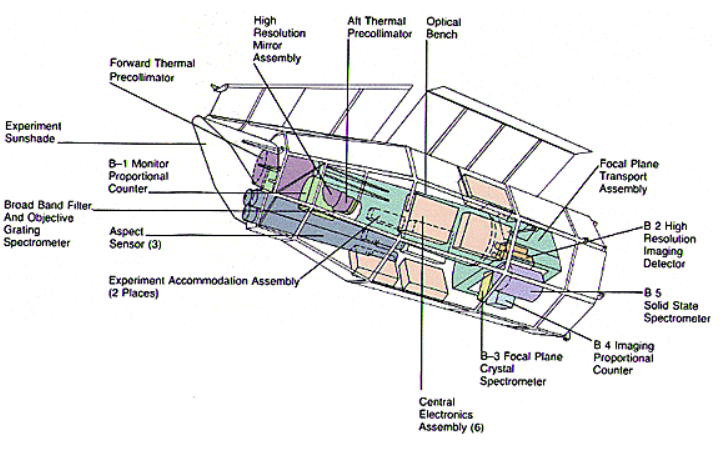
\includegraphics[scale=1]{images/einstein.png}}
\caption{Schematic of the Einstein Observatory from \cite{giacconietal1979}. }
\label{imbeded_fb}
\end{figure}


\subsection{Einstein's Design}

The telescope’s design was a Wolter type I design, which used a parabolic primary mirror followed by a hyperbolic secondary. 
The geometry of such a design (shown in Fig. 2.2) uses grazing incidence optics to reflect X-ray photons at very shallow angles towards one focal point. 
The grazing angle required to successfully reflect X-rays in 0.2-4 keV band was about 1$^{\circ}$.
By nesting several mirror shells with the same focal plane, the collecting area was increased without causng much loss in resolution.
Therefore, the Einstein telescope consisted of 4 nested reflecting surfaces with the innermost and outermost surfaces having a diameter of 33cm and 56cm, respectively.
This mirror design resulted in an effective area of 400 cm$^2$ at 0.25 keV and 30 cm$^2$ at 4 keV. 
It provided an angular resolution of 5’’ on axis but 1.5’ at the edge of the 1 degree field of view \citep{giacconietal1979}.

\begin{figure}[H]
\centering
\scalebox{0.8}{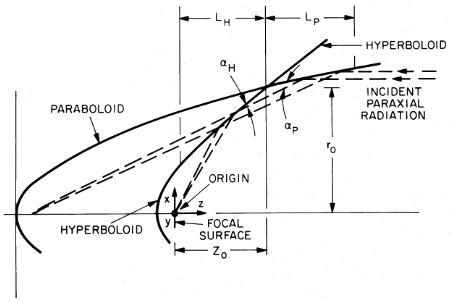
\includegraphics[scale=1]{images/einstein_wolter_type_one_design.png}}
\caption{The geometry of the Wolter type I X-ray telescope design from  \cite{giacconietal1979}. }
\label{imbeded_fb}
\end{figure}


\subsection{Einstein's Instruments}


 In the telescope, there were four main instruments that it carried: the Imaging Proportional Counter (IPC), High Resolution Imager (HRI), the Solid State Spectrometer (SSS), and the Focal Plane Crystal Spectrometer (FPCS). 
 Of the four, the IPC was the most widely used. 
 The IPC was a gas-filled detected that contained electrodes arranged with an anode in between two cathodes. 
 The anode is accelerated by X-ray photons. 
 It then discharges and sends an induced signal to the cathodes. 
 This allowed the IPC to determine the position of an event to 1 arcmin accuracy over a 60 x 60 arcmin FOV. 
 However, the centroid of the point source was determined to greater precision than 1 arcmin. 
 The IPC had a field of view of 75’ x 75’ but had less position precision 1 arcmin at the periphery of this field of view.
 It has a angular resolution of 1’, an effective area of 100 cm$^2$ at $\sim 1$ keV, and operated in the 0.15-4 keV energy range \citep{giacconietal1979}.


 
 \subsection{X-Ray Surveys with Einstein}



One of Einstein’s most notable scientific achievements was the detection of thousands of serendipitous sources.
That is, in observations of a target object, objects in the periphery are also detected due to its large field of view.
A fairly large portion of the sky was in each IPC observation, which made partial sky surveys possible.
Due to the nature of the serendipitous sources, these catalogs are dependent on how the data is interpreted and processed.
Different biases and source detection methods can lead to different sources being considered real or spurious.

The Medium Sensitivity Survey (MSS; Gioia et al. 1986) used the IPC to create a sample of 680 sources at high latitude sky using 1160 IPC images. 
This totaled a sky coverage of 590 deg$^2$.
The sensitivity of the MSS ranged from $5\times 10^{-14}$ to $3\times 10^{-12}$ erg cm$^{-2}$ s$^{-1}$ in the 0.3 - 3.5 keV energy band.
The selection process of the MSS also considered only the inner $60' \times 60'$ field of view of an image and considered sources with a signal-to-noise ratio (SNR) greater than a 5$\sigma$ threshold.
It also omitted IPC fields that were within 20 deg of the Galactic plane in order to safely assume a neutral hydrogen column density of $3\times 10^{20}$ cm$^{-2}$. 
Ultimately, the MSS was used to construct an X-ray selected quasar sample.

The efforts of the MSS were later expanded in the Einstein Extended Medium Sensitivity Survey (EMSS; Gioia et al. 1990).
The EMSS had a primary goal of detecting different populations of discrete sources responsible for the X-ray background.
Like the MSS, the EMSS included sources to the same sensitivity range and also enforced the same position restriction ($|\text{b}| >$ 20 deg). 
The EMSS, however, re-analyzed all the IPC image fields to exclude only fields that were centered on bright sources and/or extended sources.
It also excluded fields containing groups or association of objects. 
The EMSS lowered their SNR threshold to 4$\sigma$.  
As a result, the  EMSS contained 835 sources from 1435 images  from the improved calibration techniques which gave a total sky coverage of 778 sq degrees of high latitude sky  \citep{gioia1990}.

In order to incorporate the faintest sources from Einstein (and fainter sources that those found in EMSS) \cite{moran1996} constructed a new catalog using Einstein’s IPC field images which included sources exceeding an SNR threshold of 2$\sigma$.
Consequently, the catalog is named the Einstein Two-Sigma Catalog (ETS).
The primary goal of the ETS was to obtain a more complete picture of the components of the cosmic X-ray background.
In order to do this, different criteria were employed to select IPC fields.
First, the ETS excluded all images centered on sources of bright, diffuse emission as these are objects likely to contain a high concentration of spurious 2$\sigma$ sources.
Sources within 10 degrees of the Galactic plane were excluded with careful omission of galactic supernova remnants and fields within the Magellanic clouds.
Under these criteria, 2520 IPC images were used to construct the catalog (as opposed to 1435 images used in the EMSS). 
The IPC images (aside from the 4’ strips that lie on top of the window support ribs) used the entire 75’ x 75’ FOV of the image rather than the 60’ x 60’ FOV that MSS and the EMSS considered.
The catalog includes the target/center source as well as the sources in the periphery of each field. 
This results in a sky coverage of 1850 deg$^2$, 2.3 times that of the EMSS. 
The mean exposure times for the images was 3900 seconds while the median was 2200 seconds \citep{moran1996} .

To search for the sources in the images, \cite{moran1996} used an algorithm similar to that described in \cite{hamilton1991}. 
Using their algorithm directly resulted in uncertainties in source validity below 3.5$\sigma$.
Thus, modifications to their source-search algorithm were made. 
The source search began with the construction of two maps (one for the exposure time and another for the counts) of the IPC observations. 
Flat fielding is applied to the exposure map to account for the vignetting and gain variations in the detector wires.
The maps are combined and then a signal to noise ratio is computed for a putative source centered on each pixel.
Starting with a detection threshold of 10$\sigma$ and iteratively reducing the threshold to 2$\sigma$, any pixel that exceeds the threshold is considered a source and is then omitted in order to avoid contaminating the remaining iterations.
At lower SNR thresholds, the background annulus is increased since the minimum area used to compute the background noise becomes stricter. 
This increases the validity of the detected sources at these thresholds as it reduces the number of false sources.
Initially, 49,537 sources are detected in all of the IPC field images considered. 
After omitting the duplicates (keeping the detection with the highest SNR), 46,186 sources complete the ETS. 
Of these, 4,764 have a SNR of 3.5$\sigma$ or higher. From the soft X-ray log N($>$S) - log S relation modeling, it was determined that 28\% ( about 13,000) sources from the full ETS are real.
Below 4$\sigma$, the percentage is 22\% \citep{moran1996}. 
Thus, the ETS provides the highest number of real sources compared to the MSS and EMSS.
Figure 2.3 sows the source locations of the ETS catalog.


\begin{figure}[t]
\centering
\scalebox{0.22}{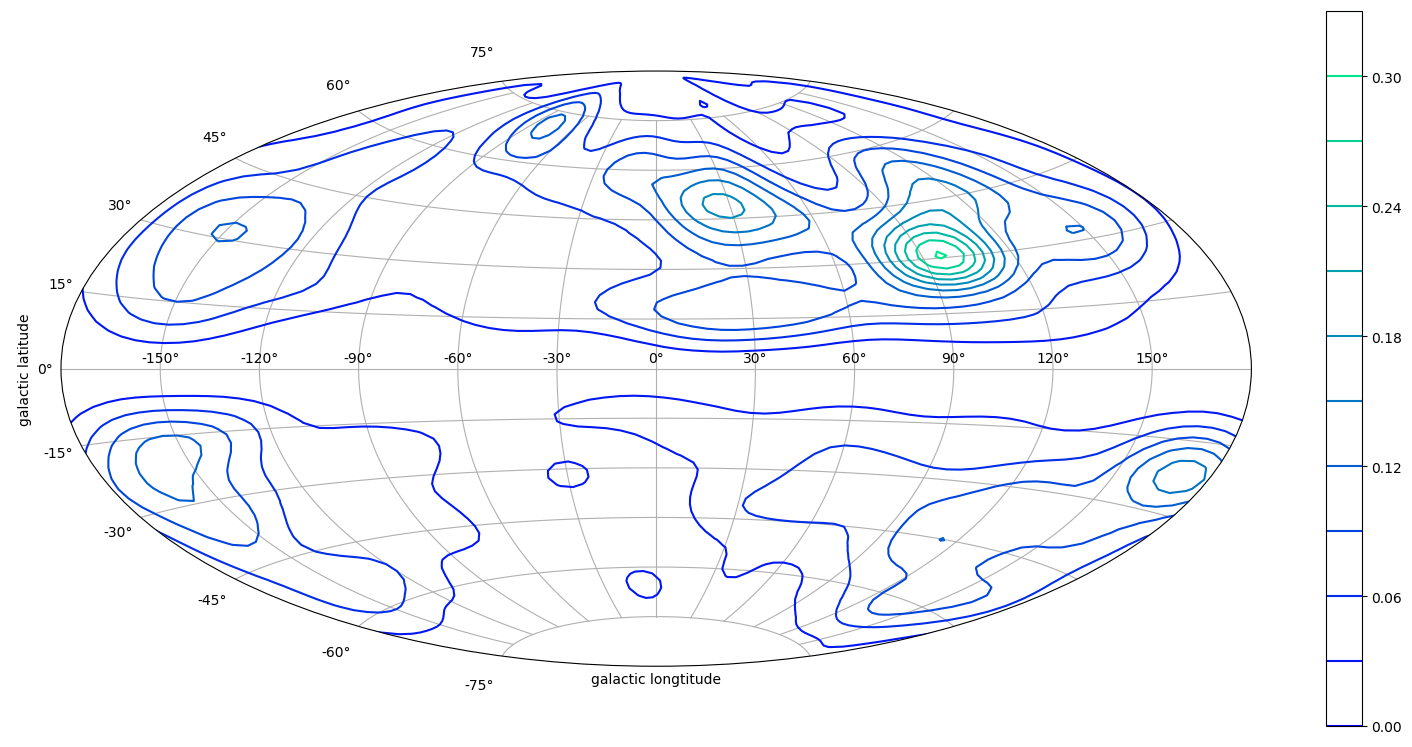
\includegraphics[scale=1]{images/ets_exp_map_contour_lines.png}}
\caption{The location of all sources from the Einstein Two-Sigma Catalog. }
\label{imbeded_fb}
\end{figure}

\FloatBarrier

\subsection{Optical Follow up of the IPC Sources}


Since the construction of the various X-ray catalogs using the IPC, optical follow ups have spectroscopically classified many of them. 
In the EMSS, the optical identification procedure involved identifying the object class based on optical spectroscopy and using the IPC X-ray flux and photometric magnitudes to compute X-ray-to-optical flux ratios, which also allows for object classification.
From this, 96\% percent of the 835 sources in the EMSS were identified. 
Of those identified, AGN made up the majority with 51.1\%. 
Galactic stars were next with 25.8\% of the catalog \citep{stocke1991}.

In the ETS, sources were optically identified by cross-correlating the data with the Green Bank 6cm and Texas 80 cm radio catalogs (where a large portion of the sources in these two radio catalogs had counterparts in VLA observations).
Allowing a separation limit of 60’’, the ETS matched to 598 6cm radio sources with a 87\% likelihood and it matched to 589 80cm radio sources with a 85\% likelihood. 
Optical spectroscopy was conducted on a few (40) of the radio-matched Einstein sources in three observing runs.
From this, the radio-selected X-ray sources was found to be mainly composed of quasars (17), with 3 of them being high redshift quasars.
At the time, one of the sources in the sample, 1508+5714, was the second most distant X-ray source known at a redshift of z = 4.30.
Other sources in the sample included ellipticals, narrow-line and broad-line galaxies, Seyferts, and liner galaxies \citep{moran1996}.

\cite{moran1996} additionally matched the ETS to the IRAS Faint Source Catalog to investigate the contribution of star forming galaxies, known to be bright infrared sources, have on the cosmic X-ray background. 
Spectra were obtained for the sample of bright infrared and X-ray sources that were a result of the cross correlation.
From spectroscopic identification of this sample, broad line AGN were found to be the dominant class.
\cite{moran1996}'s sample also found 15 new narrow-line Seyfert 1 galaxies, which characteristically have a full-width half-maximum value of H$\beta$ less than 2,000 km s$^{-1}$, a strong OIII line compared to the H$\beta$ line, and narrow FeII emission lines.
With a total of narrow-line Seyfert 1s appearing in the sample, their abundance was unexpected, but because of their known bright infrared properties, their inclusion was not.
A significant presence of star forming was not found in the sample, so evidence of them contributing to the cosmic X-ray background remained small \citep{moran1996}.



\section{The R\"{o}ntgen Satellite (ROSAT)}
\label{2_2}

The R\"{o}ntgen satellite (ROSAT;  See Fig. 2.4) was a German X-ray observatory designed at the Max-Planck Institute to carry the first all-sky suvey with an imaging X-ray telescope. 
ROSAT launched on June 1, 1990 and operated for 8 years and 8 months until its eventual demise in February 1999. 
During its mission, it was operated from the German Space Operations Center in Oberpfaffenhofen, Germany. 
ROSAT had an All-Sky Survey at the start of its mission and after, it continued through pointed observations \citep{Truemper1982}.



\begin{figure}[H]
\centering
\scalebox{0.7}{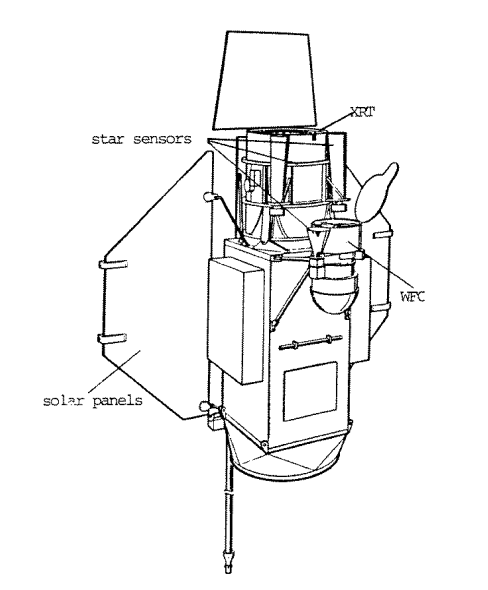
\includegraphics[scale=1]{images/rosat.png}}
\caption{Schematic of the ROSAT from \cite{Briel1996}. }
\label{imbeded_fb}
\end{figure}

\subsection{ROSAT's Design}

ROSAT was composed of two primary components: the X-ray Telescope and the Wide Field Camera. The X-ray Telescope had grazing incidence Wolter type-1 design. 
It consisted of 4 nested Wolter type-1 mirror shells.
The mirrors consisted of a zerodur substrate coated with a thin layer of gold.
The zerodur is a glass with a negligible coefficient thermal expansion and the gold coating allowed for improved X-ray reflection. at soft X-ray energies.
The optics design afforded a maximum aperture of 83.5cm and a focal length of 240cm. 
The average grazing angles for reflection occured between 1$^{\circ}$ and 2$^{\circ}$,depending on the subshell \citep{Briel1996}.

The Wide Field Camera has 3 nested mirrors (seperate from the XRT’s mirrors) in a Wolter-Schwarzchild design. 
They were made with aluminium and also coated with a thin layer of gold and had an average grazing angle of 7.5$^{\circ}$.
It provided a collecting area of 456 cm$^2$ at 1 keV. 
This assembly had a focal length of 0.525 meters. 
The instruments at the focal plane consisted of a curved microchannel plate and a carousel with 8 filters. 
The Wide Field Camera had a 5$^{\circ}$ field of view with a spatial resolution of 2.3'.


\subsection{The XRT's Instruments}

The X-ray Telescope had two imaging instruments at its focal plane: the Position Sensitive Proportional Center (PSPC) and the High Resolution Imager (HRI). 
Of the two, the PSPC was more widely used. It consisted of four componentes: PSPC-A, PSPC-B, PSPC-C, and PSPC-D, each 8cm $\times$ 8cm in size \citep{Truemper1982}. The PSPC-A and PSPC-D were only used for ground calibrations and were spares during ROSAT's mission.
They are all multiwire proportional counters where each electrode (anode and cathode) is a wire grid. 
The grids were inside of a counter filled with gas which had the following mixture: 65\% argon, 20\% xenon, and 15\% methane.
PSPC-C was meant to be the primary detector for ROSAT’s mission (and operated as such for most of ROSAT’s All Sky Survey) until the telescope scanned the sun, which destroyed the detector. 
Afterwards, the PSPC-B carried on with the mission and was used for all of the pointed observations. 
The PSPC had a 2$^{\circ}$ diameter field of view,  a spatial resolution of 0.25’ at 1 keV, and an effective area of 240 cm$^2$ at 1 keV. 
It operated in the 0.1 - 2.4 keV band.
The PSPC provided higher sensitivity, better spatial resolution, and lower background noise (from instrument and sky) than Einstein \citep{Belloni1994} .

\subsection{The ROSAT All-Sky Survey}


As mentioned earlier, ROSAT was launched with the intent of carrying out the first imaging all sky survey in the soft X-ray band (0.1-2.4 keV). 
The ROSAT All-Sky Survey (RASS) was a six month mission from July 1990 (a few weeks after its launch) until January 1991. 
During this survey period, the sky was scanned in great circles of 2$^{\circ}$ strips which intersected at the ecliptic poles. 
The total exposure time of the survey was 1.031 x 10$^7$ seconds (119.36 days) but the exposure time varied widely by region in the sky (see Fig 2.5 showing the exposure map of the RASS). 
Because of the way the RASS scanned the sky, the ecliptic equator averaged 400 seconds of exposure time while the ecliptic poles had a maximum exposure of 40,000 seconds \citep{voges1992}.




\begin{figure}[H]
\centering
\scalebox{0.8}{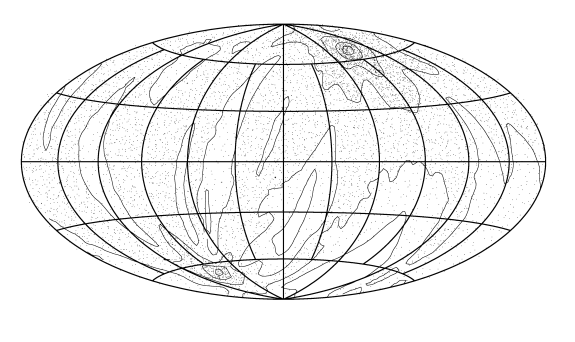
\includegraphics[scale=1]{images/rosat_all_sky_survey_exp_map.png}}
\caption{The logarithmic exposure map of the ROSAT's all sky survey where the longer exposures are darker. This projection shows the vernal equinox at the center and has right ascension (RA) increasing to the left. From \cite{Briel1996}. }
\label{imbeded_fb}
\end{figure}

The completion of the RASS mission produced a large amount of data for processing. 
\cite{voges1999} used these data to construct the ROSAT All-Sky Survey Bright Source Catalog (RASS-BSC) which picked out the brightest and most robustly detected sources from the RASS. 
To make the catalog, the 2$^{\circ}$ strips were analyzed using two source detection algorithms: a sliding window technique and a maximum-likelihood method. 

For each strip, a $3 \times 3$ pixel window moves across the photon image. 
At each of these steps, the photon count is added and compared to the background which is taken to be the 16 pixels surrounding the window. 
For extended sources, the window is increased but the background-to-source ratio of 16:9 is preserved. 
Using the sources produced from this method, circular regions with a radius equal to the window size are cut out. 
Another sliding window technique is performed and the two source lists created are merged and used as the input for the maximum likelihood method.
This method now considers each photon separately to allow for proper calibration with respect to the point spread function, which varies drastically with the off-axis angle.
The method outputs a source position and an existence likelihood. 
Finally, \cite{voges1999} selected the sources that have an existence likelihood of $\geq$ 15, at least 15 source photons, and a source count rate in the 0.1 - 2.4 keV energy band is $\geq$ 0.05 counts per second. 
After an additional screening process, the RASS-BSC had 18,8111 sources.
A similar procedure was done to generate the ROSAT All Sky Survey Faint Source Catalog (RASS-FSC; existence likelihood $\geq$ 6.5) which had 105,924 sources \citep{voges2000}.
Combining the two source catalogs produced the ROSAT 1RXS catalog.

A second, more recent ROSAT all-sky survey source catalog, called the 2RXS catalog, was constructed and released by \cite{boller2016}. 
Overall, The 2RXS catalog used similar procedures but made various improvements to them.
One of the main improvements in the 2RXS’s detection technique was that rather than using the $6.4^{\circ} \times 6.4^{\circ}$ images, it used smaller, $2.27^{\circ} \times 2.27^{\circ}$ images. 
This allowed for better determination of the local background. 
As a result, detection likelihood values are calculated with greater precision. 
Using this new improved detection method, \cite{boller2016} found that 12,000 sources in the RASS-FSC have a much lower likelihood value than originally calculated, which led them to be omitted from 2RXS. 
In total, the 2RXS has 129,192 sources (22,228 of them considered bright sources using the same criteria as the 1RXS). 
The distribution of likelihood values ranged from 6.5 to 26,198 and played a key part in the number of spurious sources. 
At a likelihood threshold of 6.5, there was a spurious detection rate of 37\%. 
Increasing the maximum likelihood threshold to 9 yields a catalog of 71,000 sources with a spurious detection rate of 5\%.
At a likelihood value of 11.01, only 1\% of the sources will be spurious. 
The exposure times of the full 2RXS catalog ranged from 7 seconds to 39,214 seconds. 
In total, the 2RXS covers 97\% of the sky with exposure time greater than 100 seconds. 

\subsection{Optical Follow Up to RASS Sources}

Once the 1RXS and 2RXS were completed, the natural progression was to optically identify the X-ray sources.
\cite{boller1992} used a subset of 14,708 extragalactic IRAS sources from the Point Source Catalog to cross correlate with the 1RXS. 
The IRAS subset was selected such that there is a strong likelihood that the source has an optical counterpart in the NASA/IPAC Extragalactic Database (NED).
Cross matching the IRAS sources and the 1RXS resulted in 244 IRAS galaxies with an X-ray counterpart from the 1RXS. 
Of these, 222 of them had optical counterparts identified by NED. 
104 of them additionally had redshifts, which allowed for the calculation of their X-ray luminosity.
The breakdown of these optically identified sources with an X-ray luminosity measurement were as follows: 50\% Seyferts, 44\% Spirals, 3\% Ellipticals, and 3\% quasars \citep{boller1992}.

In an effort to understand the role that luminous infrared sources like star-forming galaxies play in the cosmic X-ray background, \cite{moran1996} set out to obtain spectroscopic classification of the IRAS sources detected in the ROSAT All Sky Survey from \cite{boller1992}.
This was done by combining new optical spectroscopy with a thorough literature review. 
As a result of this, 210 of the sources from \cite{boller1992} were classified using new optical spectra. 
The majority of these sources turn out to be broad emission-line AGN. 
Thus, \cite{moran1996} find little evidence that starburst galaxies make up a significant portion of the X-ray background. 
In the process of classifying all of the sources, a new class of starburst/Seyfert composite galaxies was discovered. 
That is, while the optical spectra is dominated by features typical of starburst galaxies, they have X-ray luminosities typical of Seyfert galaxies. 
It is reasoned that these sources are Seyfert galaxies where their AGN component is obscured.

Additional efforts to optically identify sources in the RASS catalog include the Hamburg/RASS Catalog (HRC) by \cite{zickgraf2003} and those by \cite{gioia2003} for sources in the NEP.
The HRC was constructed by matching a patch of sky from the RASS-BSC ($\left|\text{b}\right| \geq$ 30$^{\circ}$ and dec $\geq$ 0$^{\circ}$) totaling 5341 X-ray sources with the Hamburg Quasar Survey.
This resulted in 82\% of 5341 sources being identified. AGN made up the large majority of the X-ray sources (42\%) followed by sources with stellar counterparts, which represented 32\% \citep{zickgraf2003}. 


\cite{gioia2003} focused on optically identifying sources in the NEP.
This was done in an extensive program that lasted 9 years (1991 - 2000) to observe the 445 sources from RASS in the NEP. 
Most of the observing was done at Mauna Kea (100 nights of observing) with a few observations at the University of Hawaii’s 2.2m telescope, the Canada-France-Hawaii 3.6m telescope and the Keck 10m telescope. 
In the end, after obtaining all the spectra needed, \cite{gioia2003} were able to identify 99.6\% of the sources and determine redshifts for the extragalactic ones.
The breakdown of classifications is similar to the results of \cite{zickgraf2003}.  
\cite{gioia2003} found 49\% of sources to be AGN (both type 1 and type 2) followed by 34\% of sources which had stellar counterparts. 
Clusters and groups of galaxies made up 1\% of the sources observed \citep{gioia2003}.




\section{The Chandra X-ray Observatory}
\label{2_3}


Originally called the Advanced X-Ray Astrophysics Facility when proposed by R. Giaconni, the Chandra X-ray observatory (shown Fig. 2.6) is one of NASA’s Great Observatories alongside the Hubble Space Telescope, the Compton Gamma Ray Observatory and the Spitzer Space telescope. 
Chandra launched on July 23, 1999 in the Space Shuttle Columbia with an initial planned mission of five years. 
At the time of this writing, Chandra’s mission is still ongoing, having a mission life of more than 20 years now.


\begin{figure}[H]
\centering
\scalebox{0.55}{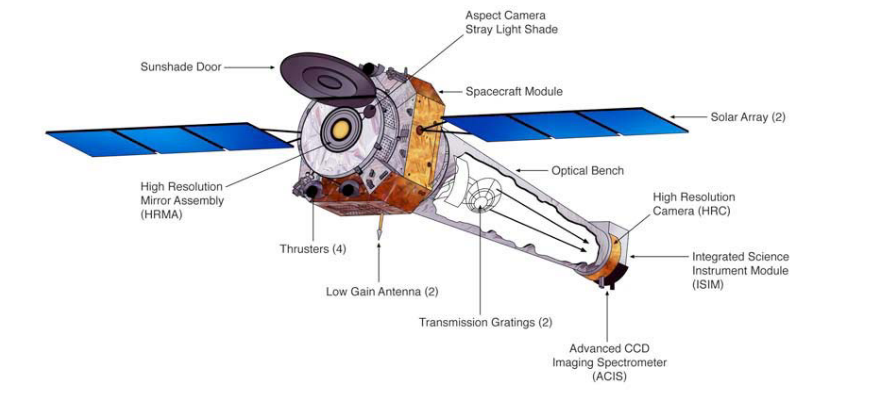
\includegraphics[scale=1]{images/chandra.png}}
\caption{Schematic of the Chandra X-ray Observatory from \cite{weisskopf1999}. }
\label{imbeded_fb}
\end{figure}

\subsection{Chandra's Design}

The Chandra X-ray Observatory’s mirror assembly design is the same as that of Einstein and ROSAT.
That is, it uses a Wolter type 1 design with 4 nested reflecting mirrors. 
All mirrors have a thin coating of iridium, which has a greater reflectivity than gold at most  X-ray photon energies. 
This results in typical grazing angles of 27’ to 51’. 
The aperture diameter of the outermost mirror is 1.2 m. 
With a focal length of 10m, Chandra has an on axis resolution of 0.5’’.
At 1.5 keV, the effective area falls fairly linearly as a function of off-axis angle, retaining 80\% of the effective area at an off-axis angle of 14'.
At higher energies, the off-axis angle affects the effective area more dramatically.
At 9.7 keV, an off axis angle of 14' reduces the effective area by 20\% \citep{weisskopf2002}. 

\subsection{Chandra's Instruments}

The primary instruments of the Chandra Observatory include the focal plane science instruments and the objective transmission gratings. 
At the focal plane, Chandra carries the Advanced CCD Imaging Spectrometer (ACIS) and the High Resolution Camera (HRC). 
ACIS is made of two CCD arrays: a 4-chip array in a  $2 \times 2$ configuration, called ACIS-I and a 6-chip array in a $1 \times 6$ configuration, called ACIS-S. 
The schematic of the ACIS focal plane is shown in Fig. 2.7. 
Each CCD has $1024 \times 1024$ pixels, with each pixel having a size of 23.985 microns. This results in a $8.3' \times 8.3'$ size for each CCD. 
Thus, the ACIS-I has an array size of $16.9' \times 16.9'$, and ACIS-S has an $8.3 \times 50.6'$ array size. 
The ACIS-I is made up of four front illuminated CCDs  while the ACIS-S is made up of two front illuminated chips and four back illuminated CCD chips \citep{weisskopf2002}.


\begin{figure}[H]
\centering
\scalebox{0.6}{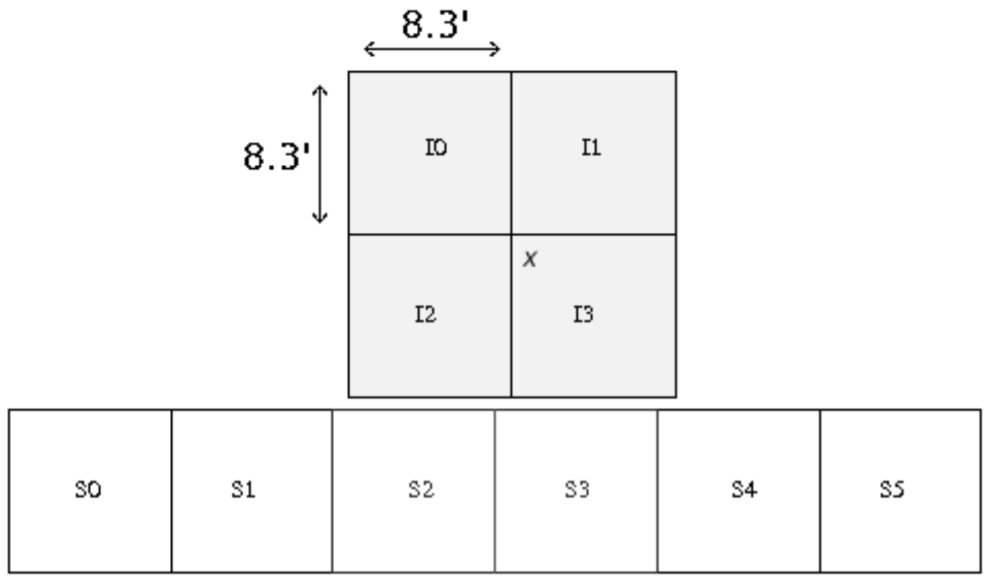
\includegraphics[scale=1]{images/chandra_acis_chips.png}}
\caption{Schematic of the Chandra's ACIS chips from \cite{weisskopf2002}. }
\label{imbeded_fb}
\end{figure}


Various configurations of ACIS are possible and each is better suited for different scientific uses. 
Using the labels used in Fig. 2.7, common configurations include the wide field imaging which uses all of ACIS-I (I0-I3) and the S2-S3 CCDs from ACIS-S.
This gives a field of view of $16.9' \times 16.9'$ plus $8.3' \times 16.9'$.
Another common configuration is the high resolution imaging which only uses the back illuminated S3 CCD without having to use any of the gratings. 
This provides a field of view of $8.3' \times 8.3'$.
In the 1-CCD chip mode, it is possible to subarray the chip to smaller dimensions. 
Typical subarrays restrict the CCD chip to 1/2, 1/4, or 1/8 of the original chip size in one dimension.
This reduces the field of view in that dimension to roughly 4', 2', or 1', respectively.
\citep{weisskopf2002}.

The other focal plane science instrument is the HRC, which is a microchannel plate (MCP) instrument also with two detectors: the HRC-I and the HRC-S. 
The HRC-I provides a field of view of $30' \times 30'$, the largest field of view of any Chandra detector. 
Thus, the HRI-I is used for wide-area imaging. The HRC-S is used for high resolution spectroscopy.

Lastly, Chandra has two transmission grating spectrometers, which are gold gratings that are placed behind the mirrors. 
The grating that is optimized for low energies  (0.07 - 0.2 keV) is called the Low Energy Transmission grating (LETG) and the other, which is optimized for higher energies ( 0.4-10 keV) is called the High Energy Transmission Grating (HETG).

\subsection{Chandra Souce Catalogs}

With the intent of providing a definitive catalog of the X-ray sources detected by Chandra, \cite{evans2010} constructed the Chandra Source Catalog (CSC).
The CSC was constructed largely using the ACIS-I, ACIS-S, and the HRC-I observations taken from the first eight years of Chandra’s mission. 
Recently, however, the second version of the CSC, called the CSC2.0, was officially released using similar but improved source detection methods as the CSC. 
This updated version included detections through the end of 2014 \citep{Evans2020}.

The CSC2.0 (just like CSC) was created using an automated data analysis and source detection pipeline.
The detection process started by using the observation IDs (image fields) to filter out observations that were conducted using the HRC-S, any grating observations, and any that included solar system and/or moving targets. 
This left most ACIS-I, ACIS-S, and HRC-I observations. 
Each one of these observations are then stacked with other observations that observed the same field of view, have a similar aimpoint (less than 1 arcmin so that the point spread function can be reliably combined), and were observed with the same instrument. 
For each stack, a pre-detection method picks out the brightest sources in each stack.
These sources are used in a “fine astrometry correction” step where the corrections needed to properly align the stacks are calculated. 
This results in having stacks that are aligned together up to less than a pixel and have more cohesive aspect solutions. 
For each observation in each stack, background flares candidates are removed from the observation to improve signal-to-noise ratio of the sources.
Full field background maps are then created and are used to simulate the counts necessary to detect a source.
The files are combined back into the stacks and combining with the background maps, an initial list of potential sources are created. 
A series of source-validation and maximum existence likelihood algorithms are used to verify the sources. 
Master match detections are created by stacking observations that overlap despite being from different instruments or having aimpoints separated by larger than 1 arcmin.
These are called the master sources and are given 2CXO catalog names. 
The CSC2.0 releases the detections found in each observation ID, in the stack observations, and in the master matches \citep{Evans2020}.

In total, the CSC2.0 includes information for 317,167 unique sources.
This was done using 928,280 individual observation detections from 10,382 ACIS and HRC-I images. 
This results in the source location map shown in Fig. 2.8. 
The false source rate is roughly 0.1 false source per field. 
The exposure times range from 0.6 ks to 5.9 Ms, with a median exposure of 12 ks.
There is a total sky coverage of 520 deg$^2$ in the B (Broad) band (0.5-7.0 keV) and 55 deg$^2$ for the W (Wide) band (0.1-10 keV) for the HRC \citep{Evans2020}.



\begin{figure}[H]
\centering
\scalebox{0.35}{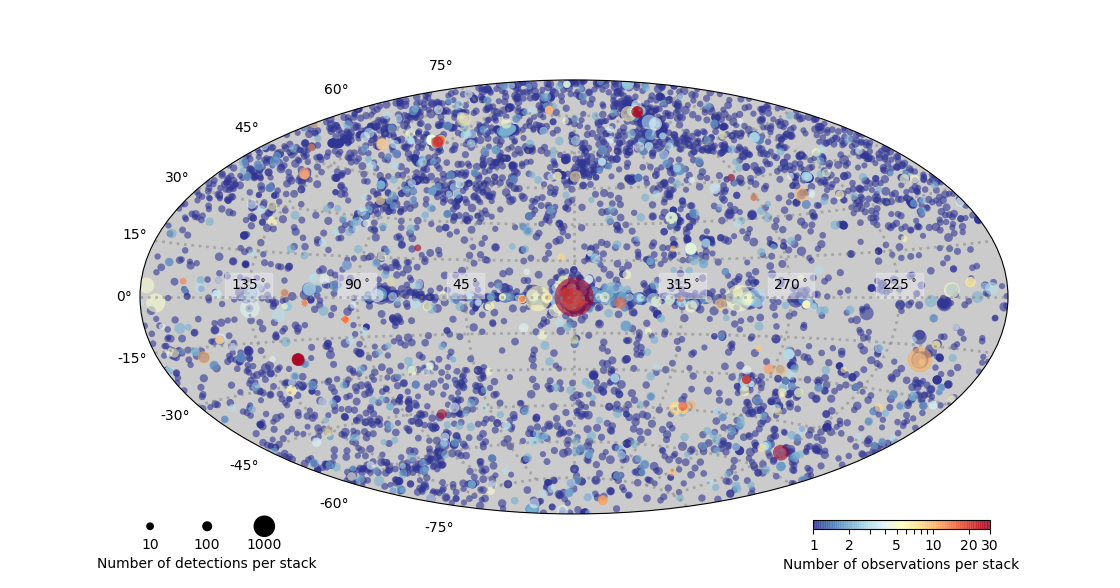
\includegraphics[scale=1]{images/csc2.png}}
\caption{Exposure map of the Chandra Source Catalog version 2.0 from \cite{Evans2020}. }
\label{imbeded_fb}
\end{figure}


\subsection{Optical Follow Up to Chandra Detections}

Since the CSC and CSC2.0 are relatively new and on-going catalogs that will likely be updated in future data releases, there are not many completed projects aimed at optically characterizing the sources in the catalog. 
However, efforts to characterize patches of sky observed by Chandra have been made for specific scientific goals. 
Of them, one of the larger projects (in terms of sky coverage) is the Chandra Multi-wavelength Project (ChaMP) survey \citep{kim2004} and the  Chandra Multiwavelength Plane (ChaMPlane) survey \citep{grindlay2005}.

The ChaMP survey cataloged serendipitous Chandra X-ray sources in a 14 deg$^2$ area.
The goal of the survey was to obtain samples of high redshift AGN and galaxy clusters \citep{kim2004}.
This catalog contained 486 X-ray sources. 
Optical follow up to these sources was conducted by \cite{green2004} where they found counterparts for 377 (78\%) of the sources. 
Obtaining spectra from observing runs, spectroscopic classifications were presented for 125 of them as well. Of these objects, 63, roughly 50\%, were broad line AGN and 28 were galaxies with narrow line emission \citep{green2004}.




%\section{Using the Catalogs}
%\label{2_4}

%We have chosen to work with the catalogs mentioned above: the Einstein 2sigma Catalog, the ROSAT all sky survey, and the CSC2.0. 
%This allows us to maximize the detection rate as we are maximizing the sources considered and the possibility that they are observed twice throughout the three catalogs. 
%Moreover, each of the catalogs do not overlap in their mission time and our baseline covers the 40 year history of X-ray astronomy, ideal conditions for studying long-term, dramatic X-ray variability.





\chapter{X-ray Sources in Multiple Source Catalogs}
\label{chap3}

Despite the fact that imaging X-ray astronomy has had a short history compared to other sub-fields, X-ray missions have provided plenty of data and source catalogs. 
Some of those were highlighted in the previous sections. 
We set a goal of finding X-ray data that spans the longest baseline possible.
Therefore, we choose to work with the Einstein Two- Sigma Catalog (ETS), the Second Rosat All Sky Survey (2RXS), and the second release of the Chandra Source Catalog (CSC2.0). 
Comparing the catalogs, however, is not as simple as it may appear. 
This is largely due to the varying optical capabilities of each telescope.

\section{Comparing Telescope Optics}
\label{sub3_1}

Because Einstein, ROSAT, and Chandra all had different scientific goals and because they were constructed at different points in time, their telescope optics differ drastically in certain respects. 
However, they all also have components that are similar to each other. 
One main component that is the same is the mirror assembly of each. 
As could have been noted from the previous sections, all telescopes have a grazing incidence Wolter type 1 mirror assembly.
Einstein’s had a diameter of 56 cm, ROSAT had a diameter of 83.5 cm, and Chandra’s is 1.2 m.

Because of technological advances that have been made between the time Einstein and Chandra, the manufacturing of the optics plays a key role in the differences between the telescopes as well.
The surface of ROSAT's mirror was smoother, with roughness variations on micron scales, than those on Einstein. 
Chandra comes closer to achieving an ideal surface than ROSAT, so the center of the Chandra's PSF is narrower than the PSF for ROSAT. Additionally, the gas-filled IPC and PSPC detectors do not localize events as well as a CCD, so the PSF of the Einstein and ROSAT are broaden even more.

Another important comparisons can be made from each of the telescopes instruments that were used to construct the catalogs that are being considered. 
For the ETS, Einstein’s IPC focal instrument was used, ROSAT used the PSPC, and Chandra largely used ACIS-I. 
Chandra’s ACIS instrument is more detailed, more sensitive, and provides the finest spatial resolution of the three.
ROSAT has worse spatial resolution than Chandra but has the largest field of view of the three instruments.
Table 3.1 displays these properties for the instruments. 
These properties result in source position uncertainties that are very different. 
In fact, the source position uncertainties for the ETS and the 2RXS are much more substantial than those for the CSC2.0.


\begin{table}[H]
    \centering
    \begin{tabular}{cccc}
    \hline
    \hline
          &Resolution & Field of View & Effective Area (at 1 keV) \\
         \hline
        Einstein IPC    & 1'&$75' \times 75'$   & 100 cm$^2$ \\
        %
        ROSAT PSPC    &  0.25'  &  $2^{\circ}\times 2^{\circ}$ & 240cm$^2$  \\
        %
        Chandra ACIS & 0.5'' & $16.9' \times 16.9'$ & 340 cm$^2$ \\
    \hline
    \hline
    \end{tabular}
    \caption{Properties of the focal instruments on the Einstein \citep{giacconietal1979}, ROSAT \citep{Briel1996}, and Chandra \citep{Evans2020}.}
    \label{tab:my_label}
\end{table}

One major component that these surveys have in common (and the main reason why they were chosen) is the energy bands in which they are most sensitive. Einstein’s IPC operated in the 0.16 - 3.5 keV energy band, the PSPC in the 0.1 - 2.4 keV band, and  Chandra’s ACIS in the 0.3-8 keV band. 
A range where they are all sensitive (and the range which was selected to calculate flux values) is the 0.5 - 2.0 keV band. 
Thus, from the properties presented, it is clear that comparisons (handled with extreme care) can be made for these catalogs as well as the fluxes of the sources they contain. 

This chapter describes the methods by which we cross matched the three source catalogs. 
Early iterations cross matched only the ETS with the CSC2.0, but because of the drastic differences in their angular resolution and field of view, there was low confidence in true matches.
Chandra is able to resolve multiple sources in a dense patch of sky while Einstein's source position uncertainty does not allow us to say which source exactly Einstein observed or if observed the cumulative diffuse emission of the dense region. 
For this reason, on many occasions, an observation of what was thought to be a discrete point source by Einstein is resolved as galaxy cluster by Chandra.
To increase reliability, the 2RXS catalog is used an intermediate step since the ROSAT's optics are more comparable to Chandra's optics.
Thus, we start by comparing the ETS and the 2RXS.
This adds confidence in ETS sources since the 2RXS's source position uncertainty is considerebly better.
We use that matched listed to cross correlate it with the CSC2.0 using both the ETS and the 2RXS source positions and position uncertainties. 
We also look for ETS sources that were not found in the 2RXS in the CSC2.0.

\FloatBarrier

\section{ETS-2RXS Catalog Matching}

To ensure that all possible matches are accounted for, every source in the ETS catalog is compared to every source in the 2RXS catalog. 
For every match pair, a “normalized offset” is computed. 
The normalized offset is given by the following equation, which takes into account the separation of the sources and 1$\sigma$ position uncertainty  of the 2RXS and the ETS source:

\begin{equation}
    \text{normalized offset} = \frac{r}{\sqrt{\sigma_{ \text{IPC} }^2  + \sigma_{ \text{2RXS}}^2 }    }
\end{equation}

Sources that are close to each other (compared to their combined source position errors) will thus have a small normalized offset value while those that are farther away  (which are less likely to be true matches) will have a much larger normalized offset value. 
Therefore, this value can be used to asses the probability that the ETS - 2RXS source matches are true or spurious matches. 
Before choosing a normalized offset value as the cutoff for true matches, general match statistics involving all possible match pairs are computed and considered. 
This helps in creating a more sophisticated approach when choosing the normalized offset cutoff value.
To find an appropriate  normalized offset cutoff value (one that will produce a list with a high fraction of true matches and minimize the fraction of spurious matches), Fig 3.1 is constructed. 

\begin{figure}[h]
\centering
\scalebox{0.7}{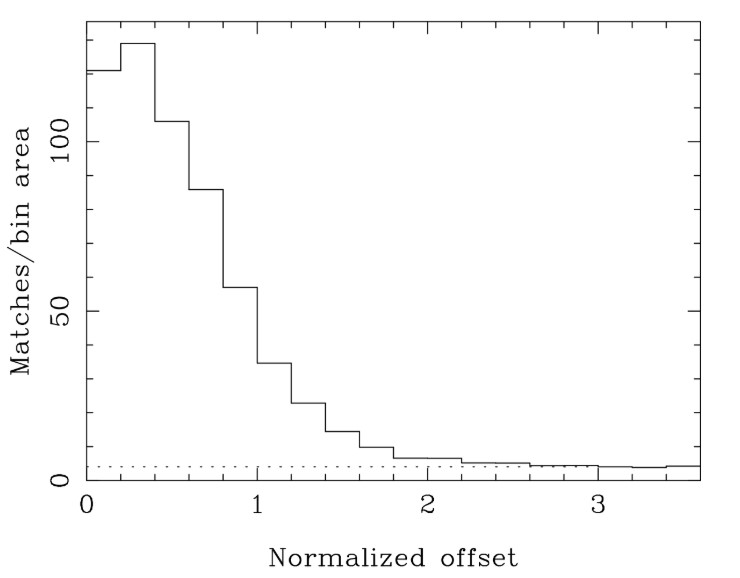
\includegraphics[scale=1]{images/ets_2rxs_match_hist.jpg}}
\caption{The density of ETS-2RXS is plotted as a function normalized offset. The background level is plotted as the horizontal, dotted line. }
\label{imbeded_fb}
\end{figure}

Fig 3.1 displays the number of ETS and 2RXS matches divided by the area of the annulus corresponding to each offset bin as a function of normalized offset.
We can expect the number of 2RXS sources that match to an unrelated ETS source at a given normalized offset away will be proportional to the area of the corresponding bin. Thus, the amount of ETS-2RXS matches that are spurious should be constant as a function of normalized offset.
That amount should then be level in Fig. 3.1.
The excess of match density area above this constant can, therefore, be associated with true matches between the ETS and 2RXS catalog.

\FloatBarrier

In Fig 3.1, the dotted line represents the expected match density due chance coincidences.
The chance coincidence level is computed by averaging the match density values of largest offset bins.
We see that almost no true matches exist beyond a normalized offset of 2.6. The density of chance coincidences allows us to determine the cumulative fraction of true matches as a function of offset (see Table 3.2).
We use this information as a diagnostic for determining a threshold for the normalized offset such that it will yield a sample of highly reliable ETS-2RXS matches.


\begin{table}[H]
    \centering
    \scalebox{0.65}{
    \begin{tabular}{cccccc}
    \hline
    \hline
         bin & number of matches &  number density &  true matches fraction & true number density   & total true matches fraction \\
         \hline
          1  & 121. &  121. &  0.967 &   117. &   0.967 \\
          2   &387. &  129. &  0.969 &  374.9  & 0.968\\
          3 &  530. &  106. &  0.962 &  509.8  & 0.965\\
          4  & 601. &   85.86 &  0.953 &  572.7  & 0.961\\
          5 &  513. &   57.00 &  0.929 &  476.7  & 0.953\\
          6  & 381. &   34.64 &  0.883 &  336.6  & 0.943\\
          7  &297.  &  22.85  & 0.823  & 244.5   &  0.930\\
          8 &  217. &   14.47 &  0.721 &  156.5  & 0.915\\
          9 &  167. &    9.82 &  0.589 &   98.4  &  0.898\\
         10  & 125.  &   6.58 &  0.386 &   48.3  &   0.879 \\        

    \hline
    \hline
    \end{tabular}
    }
    \caption{Breakdown of the match statistics from Fig 3.1 by bin.}
    \label{tab:my_label}
\end{table}

We have adopted a normalized offset cutoff of 1.4.
This yields a sample for which there is a 93\% probability the matches are genuine (only 7\% will be expected spurious matches). 
This results in a catalog of 2,824 match pairs.

After a normalized offset value of 2.6, all matches are likely to be spurious. 
For any ETS that did not match with a 2RXS source with a normal offset value of less than 2.6, the ETS source is considered a not detected in the 2RXS catalog. 
Undetected ETS sources in the 2RXS catalog are expected because of the shallower RASS exposures obtained for most of the sky.
We find that 5,210 ETS sources do not have a counterpart in the 2RXS catalog.



\section{Finding ETS-2RXS Matches in the CSC.2.0}


Now that we have identified a catalog of ETS sources that were also detecteed in the 2RXS, we can further check if they were observed in the CSC2.0. 
The cross matching, in this case, is done differently than that of the ETS and 2RXS cross matching. 
This is due to the way in which the CSC2.0 is accessed and queried.

In order to access the CSC2.0 and all its data products, we use the Chandra Viewer (CSCview).
CSCView is a graphical user interface (GUI) application developed by the Chandra X-ray Observatory that allows access to the CSC2.0 (and all other CSC releases) using user-specified queries. 
Users have the ability to choose per observation properties, stack properties, and master source properties.
To query the CSC2.0, CSCview allows users to input coordinates of one or more sources.
The crossmatch query allows users to input files containing a large number of sources.


\subsection{Initial Search}

We input our catalog of ETS sources that matched to 2RXS sources into CSCview’s cross-match function using the coordinated of the 2RXS sources, as their position errors are typically smaller than those for ETS sources.
The maximum separation allowed between a CSC2.0 source and a source in our catalog to be considered a match is a dynamic value that changes for each source. 
We use the 2.5$\sigma$ 2RXS position uncertainty as the maximum separation allowed. 
With an average 1$\sigma$ 2RXS position error of 12", the average separation allowed is 30".
Under this procedure, the CSCView's cross-matching function outputs a file with the data for all CSC2.0 sources that matched to a source from our input catalog.
Due to the different telescope optics, our results are complex. 
That is, there were 298 ETS-2RXS sources that matched to 853 CSC2.0 sources. 
This result means that there must be some ETS-2RXS sources that have more than one CSC2.0 counterpart.
Therefore, in our analysis of the source matches, we consider single and multiple CSC2.0 matches seperately.

\subsection{ETS-2RXS Sources that Match One CSC2.0 Source}

From the original results that were obtained with the CSCview, we filter to get all uniquely matched ETS-2RXS sources. That is, those for which there is a one-to-one correspondence between the ETS-2RXS catalog source and a CSC2.0 source. 
Of the 298 ETS-2RXS sources, 198 of them have only one CSC2.0 source within the 2.5$\sigma$ 2RXS position error circle. We refer to this list as the single matches list.


\subsection{ETS-2RXS Sources that Match to More than One CSC2.0 Source}

We use the original results that were given by the CSC2.0 again, but this time we are filtering to find all ETS-2RXS that were not uniquely matched. 
This means that there were more than one CSC2.0 source inside the 2.5$\sigma$ position error circle of the 2RXS source.
From the 298 ETS-2RXS sources that had CSC2.0 counterparts, 100 of them had more than one CSC2.0 that they were matched to.
Specifically, there are 100 ETS-2RXS sources that matched 655 CSC2.0 sources.
We refer to this subset of sources as the multiple matches list.

\subsection{Checking for ETS Source Ambiguity}

Using the single matches and the multiple matches lists, we go back to the CSCview. 
This time, rather than using the 2RXS coordinates and position errors, the ETS source positions and position errors are used. 
Similar to what was done in the first iteration where we the coordinates of 2RXS sources, we plug in the ETS-2RXS sources to CSCview.
Because of the poorer spatial resolution of sources in the ETS, false positives are much more likely.
Therefore, stricter criteria for what is considered a match are imposed. 

To ensure that the CSC2.0 sources that already matched an ETS-2RXS (using 2RXS position and position errors) source are being kept, the maximum separation radius is defined slightly differently. 
First, the angular separation between the CSC2.0 source that was already matched to using 2RXS data and the corresponding ETS source are calculated. 
Refer to this value as $\theta$.
The maximum separation searched for CSC counterparts is the 1$\sigma$ ETS position error or $\theta$, whichever is larger.
For the multiple matches, the largest $\theta$ value from all the CSC2.0 match correspdoing to one ETS source or that ETS's  1$\sigma$ position error is used.
Again, the largest of the two is used.
The ETS 1$\sigma$ ETS position error circle values range from 30’’ to 73’’, with an average of 47’.

\subsection{Using the Single Matches List}

We use the single matches list to find CSC2.0 counterparts using the procedure described above. 
Of the 198 sources from the single matches lists, 159 of them also produced a single match when using the ETS coordinates and position error. 
This means that the CSC2.0 source that matched the ETS-2RXS source using the 2RXS positions is the only Chandra source to match an ETS source.
In this case, we have a one-to-one-to-one match.
Figure 3.2 shows this scenario where the CSC2.0 source is within the 2.5$\sigma$ 2RXS position error and within the 1$\sigma$ ETS position error.


\begin{figure}[H]
\centering
\scalebox{0.6}{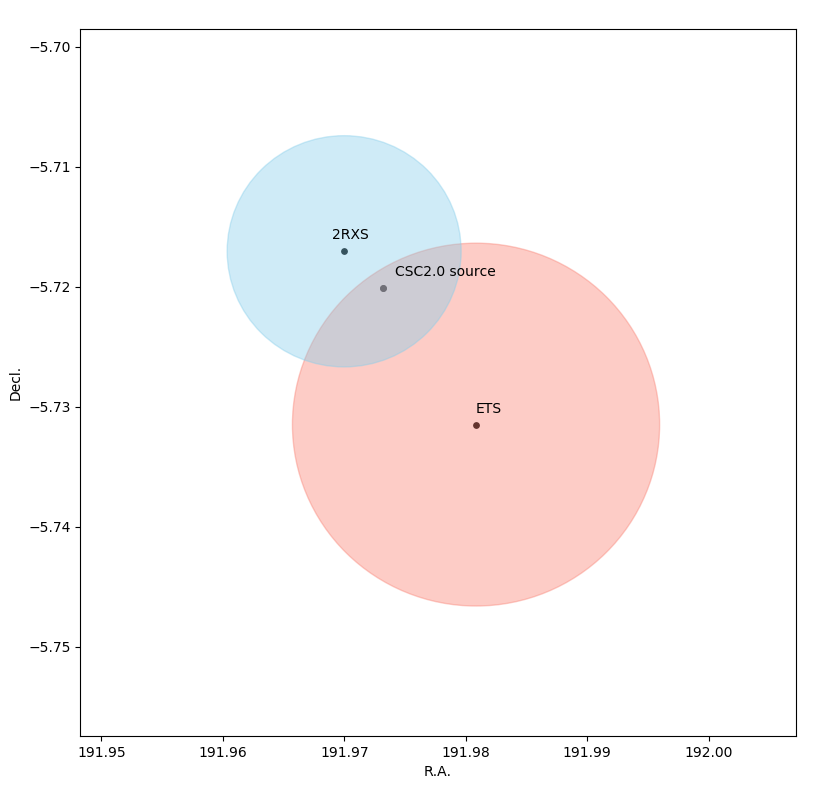
\includegraphics[scale=1]{images/ets_rass_error_circle_w_csc_source.png}}
\caption{The CSC2.0 source found in the intersection of the ETS source's position error circle and the 2RXS source's position error circle. This makes the CSC2.0 source the likely counterpart to both of these sources. }
\label{imbeded_fb}
\end{figure}

For the remainder of the single matches more than one CSC2.0 source is found within the 1$\sigma$ ETS position error. 
Specifically, 39 ETS-2RXS sources match to two or more CSC2.0 sources.
Of those 39, 25 ETS-2RXS had only 2 total CSC2.0 counterparts; 14 has more than 2.
In this case, this field of view for these sources looked similar to that of Fig. 3.3, where there is only one CSC2.0 source in the 2RXS position error circle, but there is at least one more in the ETS position error circle.

\FloatBarrier

\begin{figure}[H]
\centering
\scalebox{0.6}{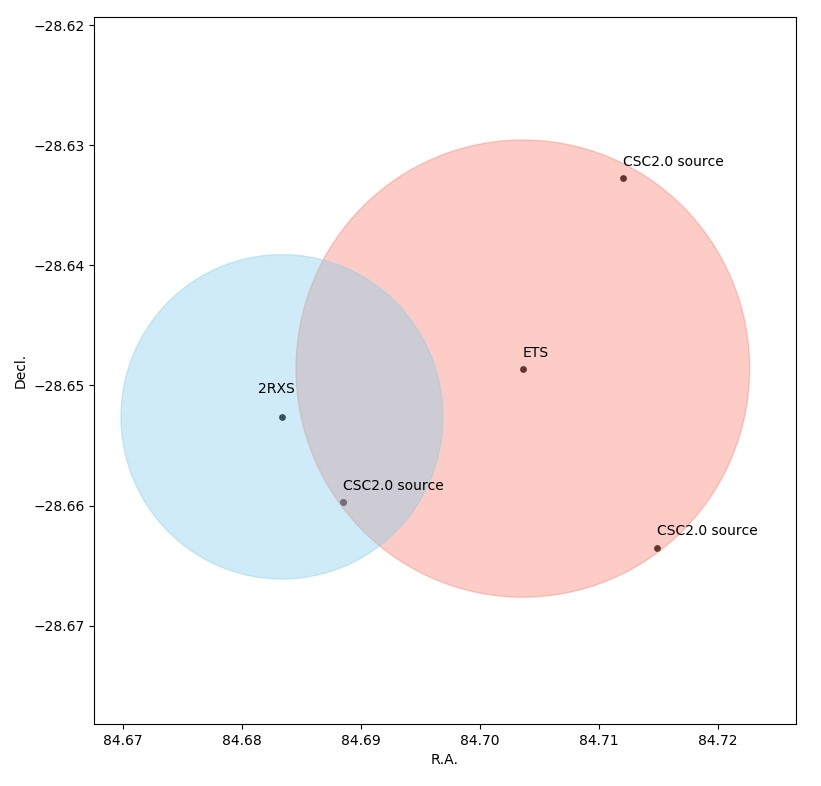
\includegraphics[scale=1]{images/single_rass_multi_ets.jpg}}
\caption{A single CSC2.0 source is found within the 2RXS position error circle but multiple CSC2.0 source are within the ETS position error circle. }
\end{figure}


\FloatBarrier

\subsection{Using the multiple matches list}

Now, we want to take a similar procedure for the multiple match lists as we did for the single match list. 
For each RASS source that matched more than one CSC2.0 sources, we now used the 1$\sigma$ ETS position errors to find CSC2.0 counterparts. 
To define our maximum separation radius, we once again define a  $\theta$ value. 
Theta is the angular separation between the ETS position and the  position of the CSC2.0 source that matched the 2RXS counterpart. 
Because multiple sources match to each of the 2RXS sources in this list, we define a $\theta_{ \text{max}  }$. 
 $\theta_{ \text{max}  }$ is the maximum theta value for any set of CSC2.0 sources corresponding to one ETS-2RXS source. 
Thus, our maximum separation value is the bigger of the following: the  $\theta_{ \text{max}  }$ value or the ETS 1$\sigma$ position error. 
Our original multiple matches list has 100 ETS-2RXS sources that matched two or more CSC2.0 sources. 
Using the ETS coordinates and the procedure just described, we find that some of those 100 ETS-2RXS sources have an additional CSC source within the ETS error circle.
Fig 3.4 shows both the 2RXS position error circle and the ETS position error circle containing multiple CSC2.0 sources.

\begin{figure}[H]
\centering
\scalebox{0.6}{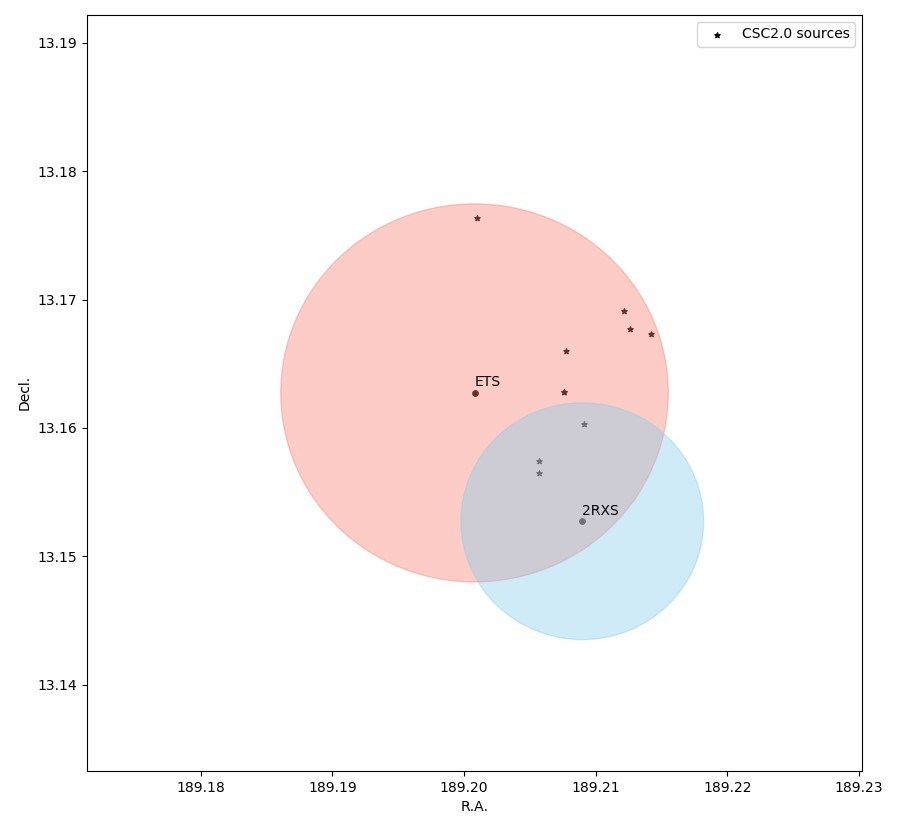
\includegraphics[scale=1]{images/multiple_multiple_pos_err.jpg}}
\caption{Multiple CSC2.0 sources found in the position error circles of the ETS source and the 2RXS source. }
\label{imbeded_fb}
\end{figure}

\subsection{Finding CSC Counterparts for ETS sources not in the 2RXS}

Of the entire ETS catalog, 5,210 of the sources with an SNR ratio above 3.0 did not have a counterpart in the 2RXS catalog. 
These sources, however, can still offer a lot of insight, so we follow a similar procedure for matching them with CSC2.0 sources to identify unambiguous matches between the ETS and CSC2.0 sources. 
Since we don’t have 2RXS to guide our identification of the CSC2.0 counterparts, the way sources are considered matches is a lot stricter. 
That is, only CSC2.0 sources that are within the 1$\sigma$ ETS position error are considered.
To remove any further ambiguity, we consider only matches that are one-to-one.
As ETS position errors can be large, the possibility that many CSC2.0 sources to lie within the position error of one ETS source is significant.
Sticking with the 1$\sigma$ position error circle allows us to be confident that the matches are real and while it is likely some real matches exist outside this radius, the probability of finding multiple CSC2.0 sources increases.
Following this procedudre, of the 5,210 sources, 202 of them matched one-to-one with a source from CSC2.0.




\section{Calculating Source Fluxes}

\subsection{ETS Fluxes}

The fluxes for the ETS sources were computed from their count rates. 
This started by obtaining the response calibration file for Einstein’s IPC instrument from the HEASARC database from NASA/GSFC. 
The response file is made up of components like the effective area curve and the detector redistribution matrix. 
An absorbed power law spectral model is assumed where the power law photon index is taken to be $\Gamma$ = 2.0 and the absorption is set equal to the galactic neutral hydrogen column density ($\text{N}_{ \text{H,gal}  }$) in the direction of a given source. 
The $\text{N}_{ \text{H,gal}  }$ values ranged from 4$\times 10^{19}$ to 3.5$\times 10^{21}$ atoms/cm$^2$.

The response calibration file and the absorbed power-law model are entered in NASA’s XSPEC, a spectral fitting software for X-ray data. 
The energy channel is restricted to the range in which Einstein’s IPC operated: 0.16-3.5 keV and a $\text{N}_{ \text{H,gal}  }$ value is selected from the above range. 
The power-law model is normalized so that XSPEC outputs the estimated count rate of 1.0 counts per second in the 0.16-3.5 keV band. XSPEC then calculates the flux based on this model in the 0.5-2.0 keV band. 

The above process is repeated for 33 different $\text{N}_{ \text{H,gal}  }$ values, all which lie in the range specified. 
With this data, a plot of 0.5-2.0 keV fluxes for 1.0 counts per second vs log($\text{N}_{ \text{H,gal}  }$) is constructed and fitted with a 5th order polynomial.
The polynomial allows us to use the measured $\text{N}_{ \text{H,gal}  }$ value of a source in the ETS catalog, and compute its 0.5-2.0 keV flux for 1 count per second. 
Multiplying by the actual count rate gives the 0.5-2.0 keV flux for the source. 
This is done for all sources in the ETS.


\subsection{2RXS Fluxes}

An almost identical approach is taken to find the fluxes of the 2RXS sources. 
The differences are due to the different properties in ROSAT’s PSPC-C instrument (which is the one that was used for the ROSAT All Sky Survey). 
Specifically, the response calibration files, of course, are different and the energy channel is restricted to an energy band of 0.1-2.4keV.
This results in a 6th order polynomial which is used to compute the 0.5-2.0 keV fluxes of the 2RXS sources.


\subsection{CSC2.0 Fluxes}

Fluxes for the sources in the CSC2.0 are calculated by the Chandra X-ray Center themselves and included as part of the data products available to query. 
The fluxes are calculated in various ways and a user can select the fluxes that best fit their needs.
The fluxes are separated in two main categories based on calculation method: aperture photometry fluxes and spectral model fluxes.

The aperture photometry fluxes are calculated for the master sources and are also calculated for all individual observations. 
For each of these sources, a “best estimate” photon and energy flux is calculated in the 0.5-7.0 keV range. 
Additionally, using the aperture source counts, an aperture model energy flux is also calculated that estimates the power law, blackbody, and bremsstrahlung model flux.

Along with aperture photometry, fluxes are calculated using spectral model fitting. 
This is done for any master source that has a high number of counts ($>$150) in the 0.5 - 7.0 keV range. 
Spectral fits are carried out for a power law model, a blackbody model, and a bremsstrahlung model. 
Each model takes different free parameters to obtain a proper fit. 
The power law model’s free parameters are the neutral hydrogen absorption column density, the power law photon index, and the power law amplitude.
The blackbody model’s free parameters are the neutral hydrogen absorption column density, the blackbody temperature, and the blackbody model amplitude. 
Lastly, the bremsstrahlung model takes the neutral hydrogen absorption column density, the bremsstrahlung temperature, and the bremsstrahlung model amplitude. 
For all the different types of ways in which the fluxes are calculated, the fluxes are reported in the broad (0.5 - 7.0 keV), ultrasoft (0.2 - 0.5 keV), soft (0.5 - 1.2 keV), medium (1.2-2.0 keV), and hard ( 2.0 - 7.0 keV) energy bands \citep{Evans2020}.

Because of how the ETS and 2RXS source fluxes are calculated and in order to have comparable fluxes, we use the aperture photometry power law model fluxes in the 0.5 - 2.0 keV (soft plus medium) energy band.


\section{Flux Ratios of Matched Sources}


With all sources in the catalogs having flux calculations, it is possible to compare the fluxes from the matched pairs that were created from the cross-matching procedure. 
Specifically, flux ratios are calculated to compare the magnitude of the change in flux between the different observations of the same source. 
The flux ratio calculation, however, is different for the singly matched sources and the match pairs with multiple CSC2.0 sources. 
Sources that display a flux ratio of more than a factor of 7 (similar to the source from the \cite{LaMassa2015} paper)  are of particular interest and are considered highly variable. 
At the end of this procedure, we generate a list of X-ray sources that appear to have undergone dramatic variability in their X-ray flux.


\subsection{Flux Ratio for Single Matches}

The flux ratio calculation of singly matched sources is the most straightforward since a direct comparison between the ETS source flux, the 2RXS source flux, and the CSC2.0 source flux can be made. 
The flux ratios are computed between the ETS and 2RXS source, the ETS and the CSC2.0 source, and the 2RXS and CSC2.0 source. 
If any of these ratios are greater than a factor of 7, we consider the source highly variable. 
From the 159 sources in the single-single matches list, 31 of the sources may be highly variable.



\subsection{Flux Ratio for Multiple Matches}

The ETS and 2RXS sources match anywhere from 2 to 10 or more CSC2.0 sources.
After a deep investigation into the matches, it becomes clear that dealing with sources that match to more than 2 CSC2.0 becomes nearly impossible.
Specifically, it is not feasible to determine how a combination of numerous CSC2.0 sources contribute to the observed ETS and 2RXS fluxes.
Thus, it is not possible to assess for X-ray variability in these cases, let alone distinguishing the source of any such variability.

However, we can and do adopt a procedure for carefully handling ETS and 2RXS sources that match to only two CSC2.0 sources.
We only consider match pairs in which (1) the 2RXS source matches two CSC2.0 counterparts within its 2.5$\sigma$ position error circle and the ETS source has no additional CSC2.0 counterparts in its own 1$\sigma$ position uncertainty circle, or (2) the 2RXS source matches to one CSC2.0 source and the ETS counterpart matches only one additional CSC2.0 counterpart.

For match pairs that correspond to first requirement, we can assume that the ETS and 2RXS observations included the flux of both of the CSC2.0 counterparts. 
To untangle the CSC2.0 sources in the ETS and 2RXS observation, consider first the flux for only one of the CSC2.0 sources. 
Let the flux of this CSC2.0 source be labeled C1 and the other flux of the other CSC2.0 source be labeled C2.
Assuming that any change in flux is entirely due to C1, we subtract off C2 from the ETS and 2RXS source fluxes.
This will yield ETS and 2RXS flux values for the CSC2.0 source that can be compared directly to the flux of C1.
Thus, we can compute flux ratios as if it were a single source.
That is, we divide the C2 subtracted ETS and 2RXS fluxes by C1 and assess for variability of the CSC2.0 source corresponding to the C1 flux value.
We can follow an identical procedure for the other CSC2.0 source to compute its flux ratios.
If any of the flux ratios is greater than a factor of 7 (or less than 1/7), we consider the source to be a candidate for high variability.
Our assumption that the change in the flux is entirely due to only one source does not allow us to consider any these sources as more than just candidates.
Following this procedure, we identify 24 match pairs that appear to be highly variable.

For match pairs that meet the second requirement, we assume that the 2RXS flux is composed of only the flux associated with the CSC2.0 source that it matched. 
Let the flux of this CSC2.0 source be labeled C1.
We also assume that the ETS flux is composed of C1 as well as the flux corresponding to the CSC2.0 source that the ETS source matched.
Let the flux for that source be denoted by C2.
Consider first the CSC2.0 source found within the 2RXS position uncertainty circle.
We can divide the 2RXS source flux and the C2 subtracted ETS source flux by C1 assess for variability.
Now consider the CSC2.0 source that is found in the ETS position error circle.
We divide the the C1 subtracted ETS flux by C2 to determine the magnitude of the flux variability.
Again, if any flux ratio is greater than a factor of 7 (or less than 1/7), we consider the source to be a candidate for high variability.
This procedure yields 22 match pairs that appear to be highly variable.

\subsection{Flux Ratio for ETS Sources Not Detected in 2RXS}

The ETS sources that were not detected in the 2RXS but have a CSC2.0 counterpart are also straightforward to compute flux ratios since we only consider the singly matched sources. 
Thus, we can compute the flux ratio between the ETS source flux and the CSC2.0 source flux. 
Among the 202 ETS sources that matched one-to-one with a CSC2.0 source, 46 of them appear to display high variability in the X-ray flux.

For all the matches that appear to have undergone dramatic variability in their X-ray flux, an investigation of their optical properties, including images and spectra, are needed to confirm whether the variability is genuine rather than an artifact related to the differing telescope instrumentation. 



\chapter{Optical Identification of Variable X-ray Sources}
\label{chap4}

From our lists of matched pairs, we have identified those which potentially exhibit dramatic variability in their X-ray flux. 
This is one half of our goal in this project. 
The other, and arguably more important, half is to determine the source of the X-ray variability.
So naturally, the next step from here is to optically identify our sample of variable X-ray sources in search of AGN.
This is done using the Sloan Digital Sky Survey (SDSS). 
SDSS is an ongoing imaging survey at optical wavelengths using the 2.5 SDSS reflector telescope at the Apache Point Observatory in New Mexico. 
Since 2000, when data collection began, the program has obtained photometric observations for one billion objects and has collected spectra of four million objects. 
To optically identify our targets, we use the SDSS data release 8 (DR8), which was released in January 2011 and covered 14,555 deg$^2$, about 35\% percent of the sky.
We look for spectra and optical images in our list of variable, unique (one-to-one-to-one) matches, in the list of variable ETS sources that had no 2RXS detection but matched to one CSC2.0 source, and the list of multiple match pairs that resulted from Section 3.5.2.
We present first the sources whose X-ray variability could be related to changes in accretion state and then sources whose variability is likely to have a different origin.





\section{Accretion Related X-ray Variability}

%%%%%%%%%%%%%%%%%%%%%%%%%%%%%
%%%%%%%%%%%%%%%%%%%%%%%%%%%%%
%%%%%%%%%%%%%%%%%%%%%%%%%%%%%

\subsection{J122934.1+134630}

J1229+1346, z = 0.099, has 0.5-2.0 X-ray flux values of 4.28$\times 10^{-13}$ \fluxunits, 5.53$\times 10^{-13}$ \fluxunits, and 6.64$\times 10^{-14}$ \fluxunits calculated from the ETS, 2RXS, and CSC2.0, respectively. 
This produces an ETS/2RXS flux ratio of 0.8724, a 2RXS/CSC2.0 flux ratio 7.76, and an ETS/CSC2.0 flux ratio of 8.33. 
Thus, J1229+1346 is considered a highly variable X-ray source from its ETS/CSC2.0 and 2RXS/CSC2.0 flux ratios, which just clear our threshold of 7. 
The SDSS spectrum of the source (Fig 4.1) presents a broad H$\alpha$ emission line with equally dominant [NII] lines on either side of it. 
The strongest line, however, is the narrow [OIII]$\lambda 5007$ line, which completely dominates over the H$\beta$ line to its left. 
These are all indicators which suggest that J1229+1346 is an AGN. 
This is, in fact, the case from BPT diagnostics conducted by \cite{puchnarewicz1992} where J1229+1346 is determined to be a Seyfert 1. 
J1229+1346 is also found in \cite{veron2006}’s extensive catalog of quasars and AGN.

\begin{figure}[t]
    \centering
    \subfloat[]{{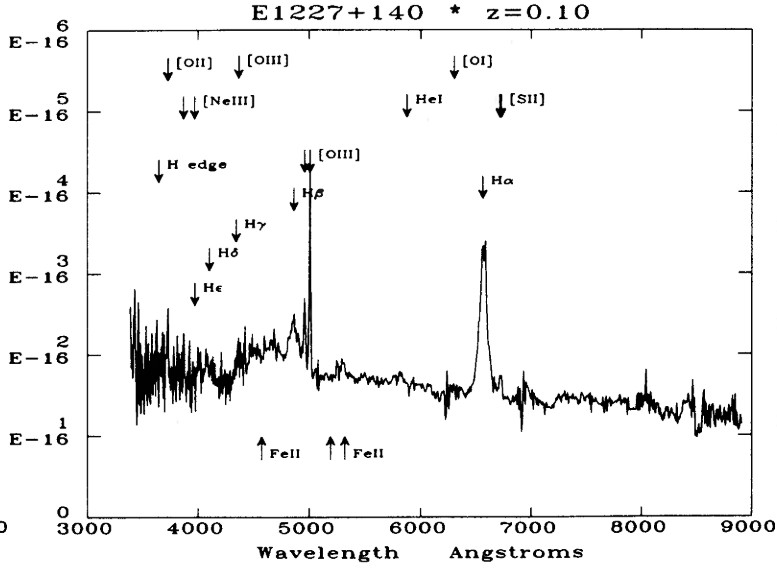
\includegraphics[width=9cm,height=5cm]{spectra/j1229+1346_spectra_paper.jpg} }}%
    \qquad
    \subfloat[]{{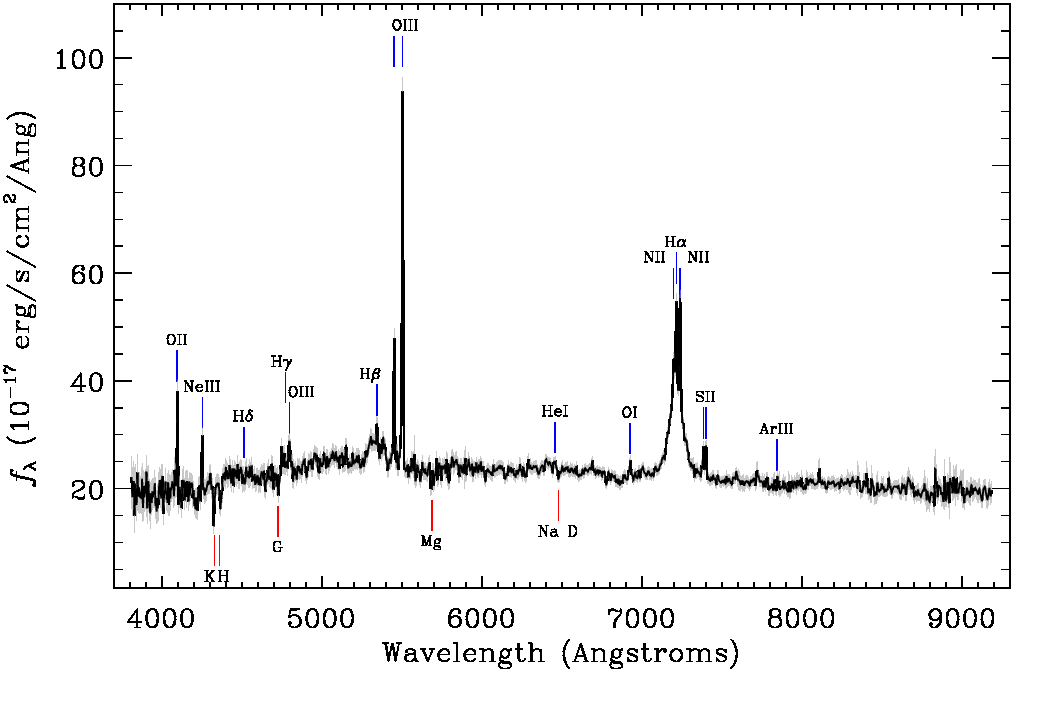
\includegraphics[width=9cm,height=5cm]{spectra/j1229+1346_spectra_sdss.png} }}%
    \caption{The spectra of J1229+1346 taken by \cite{puchnarewicz1992} in 1988 (a) and SDSS in 2005 (b). }%
    \label{fig:example}%
\end{figure}

The literature shows no evidence of some other outstanding physical characteristic which could explain the flux variability in J1229+1346. 
Therefore, it is likely that the observed change in X-ray flux is due to a change in the mass accretion rate of the AGN. 
The fluxes reveal a decrease in the accretion rate from the time of its Einstein and ROSAT observation to its Chandra observation in 2008. 
While the difference in the optical spectra obtained between 1988 and 2005 is minimal, the 1988 spectrum continuum rises to the blue while the SDSS spectrum is level with wavelength. 
This is another indicator of a decrease in activity in the AGN since it could hint at a decrease in the blue power law continuum characteristic of more luminous AGN and quasars. 
In contrast, the continuum in the SDSS spectrum appears to be dominated by starlight from the host galaxy.
The H$\alpha$ and H$\beta$ lines in the 2005 spectrum have relatively the same broadening as the same lines in the 1988 spectrum, so J1229+1346 was and is still a Sey 1.

\FloatBarrier

%%%%%%%%%%%%%%%%%%%%%%%%%%%%%
%%%%%%%%%%%%%%%%%%%%%%%%%%%%%
%%%%%%%%%%%%%%%%%%%%%%%%%%%%%



\subsection{J111520.7+404326}

J1115+4043 has an ETS 0.5-2.0 X-ray flux of 1.43$\times 10^{-12}$ \fluxunits, a 2RXS flux of 1.55$\times 10^{-13}$ \fluxunits, and a CSC2.0 flux of 4.86$\times 10^{-13}$ \fluxunits. 
This results in an ETS/2RXS flux ratio of 9.21, a 2RXS/CSC2.0 flux ratio of 2.94 and an ETS/CSC2.0 flux ratio of 0.313. 
Because of its ETS/2RXS flux ratio, J1115+4043 is considered a variable X-ray source. 
The spectrum from SDSS (shown in Fig 4.2) suggests the source is an AGN due to its broad balmer series lines and strong [OIII] and [NII] lines. 
Obtaining the spectrum and running BPT diagnostics, \cite{akiyama2003} identify the source as a Seyfert 1. 
J1115+4043 is also included in \cite{veron2006}’s catalog of AGN and quasars.


\begin{figure}[h]
    \centering
    \subfloat[]{{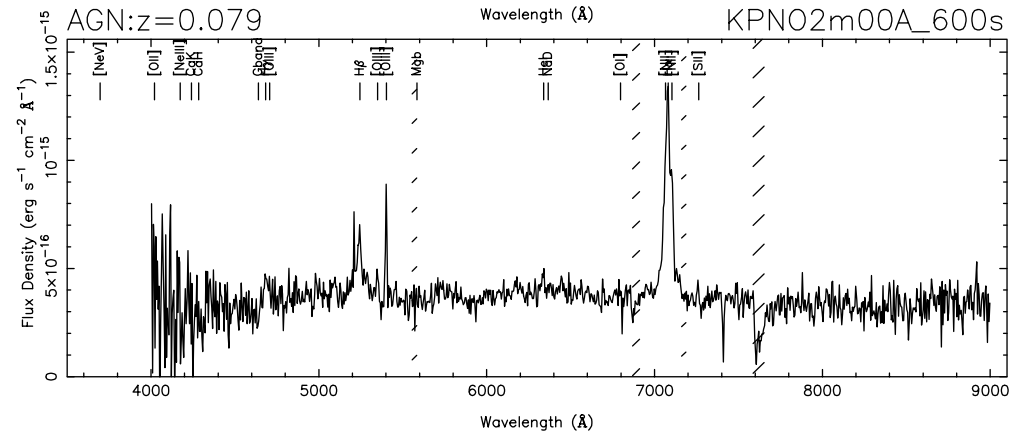
\includegraphics[width=10cm,height=5cm]{spectra/j1115+4043_spectra_paper.png} }}%
    \qquad
    \subfloat[]{{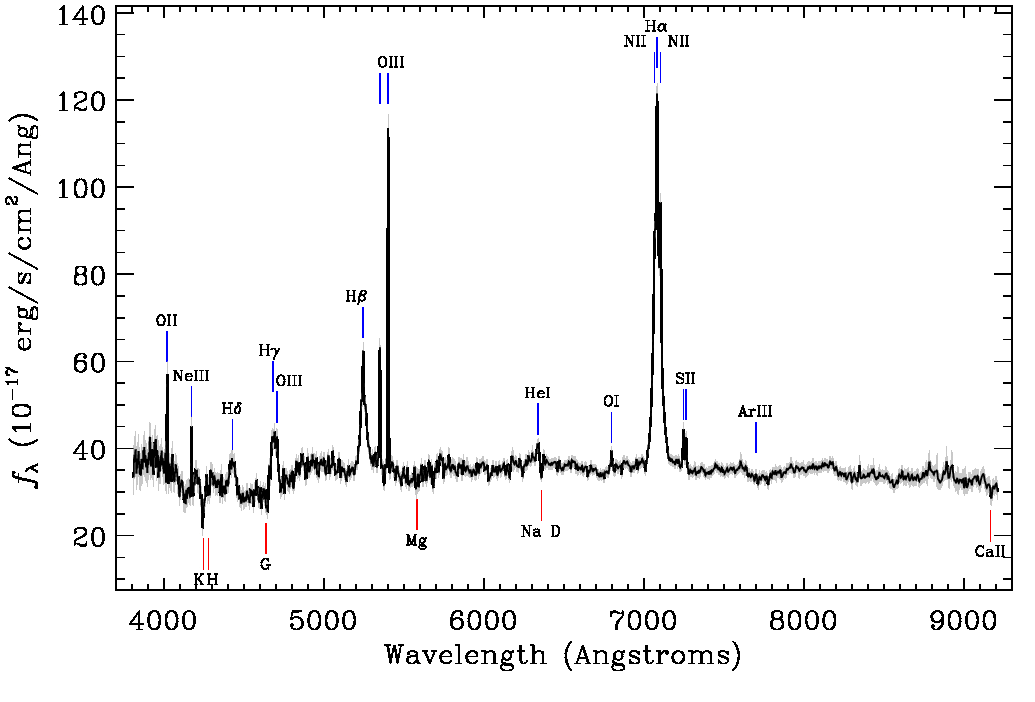
\includegraphics[width=9cm,height=5cm]{spectra/j1115+4043_spectra_sdss.png} }}%
    \caption{The spectra of J1115+4043 taken by \cite{akiyama2003} in 2000-2001 (a) and SDSS in 2003 (b). }%
    \label{fig:example}%
\end{figure}


Because the literature presents no evidence of the X-ray variability being associated with another physical phenomenon in the AGN, we can declare that the variability is likely due to a change in mass accretion rate of the AGN. 
The X-ray flux decreases significantly between the Einstein and ROSAT observations.
It then decreases slightly between the ROSAT observation and the Chandra observation, taken in 2001.
In this case, there is no difference in the optical spectrum, despite the X-ray variability.
This hints at the X-ray variability occurring before the 2000-2001 observation of \cite{akiyama2003}'s spectrum.
Therefore, both spectrum observe J1115+4043 in the same state.


\FloatBarrier
%%%%%%%%%%%%%%%%%%%%%%%%%%%%%
%%%%%%%%%%%%%%%%%%%%%%%%%%%%%
%%%%%%%%%%%%%%%%%%%%%%%%%%%%%




\subsection{J180117.9+662359}

J1801+6623, z = 1.25, has a 0.5-2.0 X-ray flux of 4.32$\times 10^{-13}$ \fluxunits, 1.38$\times 10^{-14}$ \fluxunits, and 1.87$\times 10^{-14}$ \fluxunits observed in the ETS, 2RXS, and CSC2.0, respectively.
This produces an ETS/2RXS flux ratio of 31.4 a 2RXS/CSC2.0 flux ratio of 0.73, and an ETS/CSC2.0 flux ratio of 23.07.
While J1801+6623 does not have a spectrum in SDSS, because it is near the center of the NEP region, a region that has deep exposures in the RASS, extensive information is available from multiple NEP follow up and optical identification projects. 
One of the first identifications of J1801+6623 is in the ROSAT North Ecliptic Pole Deep Survey by \cite{bower1996}. 
Here, J1901+6623 is identified as a quasar. 
It is, again, classified as an AGN in a similar ROSAT North Ecliptic Pole Survey by \cite{henry2006}. 
Both did not make their spectrum available. 
However, we obtain a spectrum of J1801+6623 (show in Fig 4.3) from an observing run at Palomar where we optically followed up on multiple ROSAT sources. 
The spectrum demonstrates a steep power-law spectrum with a broad MgII$\lambda 2800$ line, indicating that J1801+6623 is, in fact, a quasar.

\begin{figure}[h]
\centering
\scalebox{0.65}{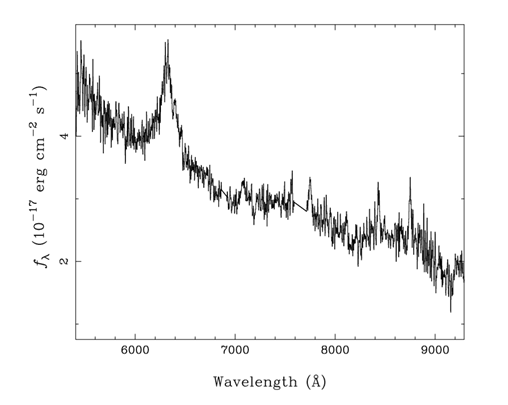
\includegraphics[scale=1]{spectra/j1801+6623_spectra_mdm.png}}
\caption{The spectrum of J801+6623 from Palomar.}
\label{imbeded_fb}
\end{figure}

While J1801+6623 has remained a quasar throughout the different observations, its X-ray flux has not remained consistent. 
Its X-ray flux decreased by a significant amount between the ETS and 2RXS observation.
Since then, it has remained constant between the ROSAT observation and the Chandra observation in 2000.
Its X-ray luminosity has remained above 1$\times 10^{44}$ ergs s$^{-1}$, which agrees with the quasar signatures present in the optical spectrum
The change X-ray flux is likely due to a change in the mass accretion rate of J1801+6623.


\FloatBarrier
%%%%%%%%%%%%%%%%%%%%%%%%%%%%%
%%%%%%%%%%%%%%%%%%%%%%%%%%%%%
%%%%%%%%%%%%%%%%%%%%%%%%%%%%%

\subsection{J082042.4+205715}


J0820+2057, z = 0.114, was not detected in the 2RXS. Ihas an ETS flux of 2.79$\times 10^{-13}$ \fluxunits and a CSC2.0 flux of 2.68$\times 10^{-14}$ \fluxunits in the 0.5-2.0 keV band. 
This produces an ETS/CSC2.0 flux ratio of 10.59, which classifies it as a variable X-ray source.
The SDSS spectrum of J0820+2057 (shown in Fig 4.4) has narrow balmer series lines, showing no initial signs of AGN activity. 
The H$\beta$ and the [OIII] lines appear to be roughly equal strength but the H$\alpha$ and [NII] lines are hard to distinguish. 
For this reason \cite{jackson2012} used the SII/H$\alpha$ line ratio in their BPT diagnostic to reveal that J0820+2057 falls in the category of star forming galaxies. 
However, X-ray observations of J0820+2057 using XMM-Netwon display a high X-ray luminosity (~10$^{43}$ in the 0.3-10 keV bad), which would make it an extremely luminous star-forming galaxy in the X-ray. 
For this reason, \cite{jackson2012} looked for other J0820+2057 physical mechanisms driving this X-ray luminosity. 
They find that J0820+2057 is a compact X-ray source, not extended, and is well fitted by a power law spectrum model, indicating that J0820+2057 is in fact an AGN. 
\cite{jackson2012} infer that the weakened  AGN component in the optical spectrum is a result of enhanced stellar emission.


\begin{figure}[h]
    \centering
    \subfloat[]{{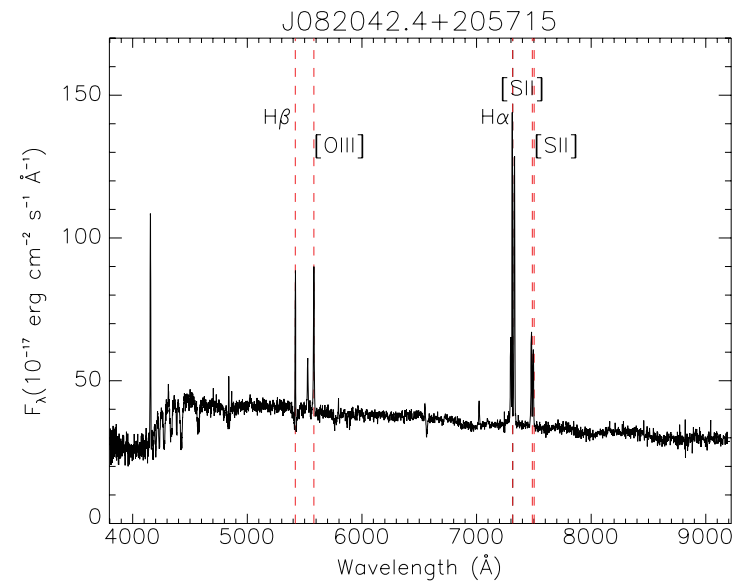
\includegraphics[width=9cm,height=5cm]{spectra/j0820+2057_spectra_paper.png} }}%
    \qquad
    \subfloat[]{{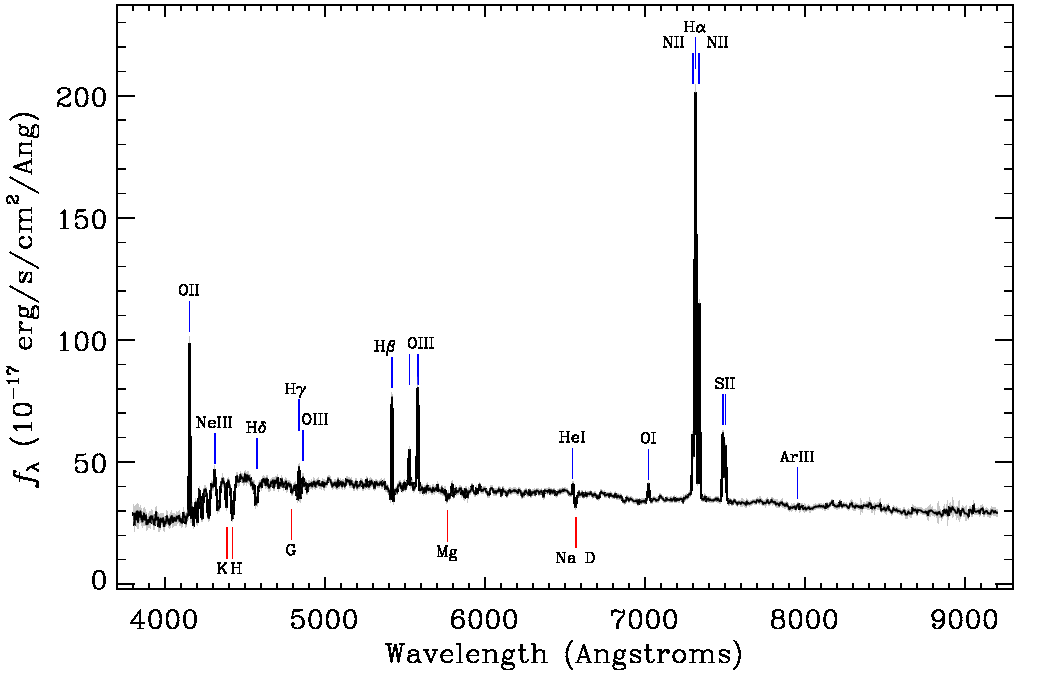
\includegraphics[width=9cm,height=5cm]{spectra/j0820+2057_spectra_sdss.png} }}%
    \caption{The spectra of J0820+2057 taken by \cite{jackson2012} in 2002 (a) and SDSS in 2004 (b). }%
    \label{fig:example}%
\end{figure}


\FloatBarrier

Optically, J0820+2057 is a peculiar source, but it appears that it is a well-behaved X-ray source. 
Thus, its X-ray variability between the ETS and CSC2.0 observations can be attributed to changes in the mass accretion rates of the AGN. 
After its initial observation with Einstein, the X-ray flux dropped significantly before it was observed with Chandra in 2007.


%%%%%%%%%%%%%%%%%%%%%%%%%%%%%
%%%%%%%%%%%%%%%%%%%%%%%%%%%%%
%%%%%%%%%%%%%%%%%%%%%%%%%%%%%

\subsection{J084309.8+292919}

J0843+2929, z = 1.51, was also not detected in the 2RXS. It has an ETS and CSC2.0 X-ray flux of 2.78$\times 10^{-13}$ \fluxunits and 1.68$\times 10^{-14}$ \fluxunits, respectively, in the 0.5-2.0 keV band. 
This produces an ETS/CSC2.0 flux ratio of 16.5, making it a highly variable X-ray source.
The spectrum for J0843+2929 (shown in fig 4.5) has broad Mg, CII, and CIV emission lines and a blue power law continuum. 
These are features characteristic of a quasar.
J0843+2929 has, in fact, been confirmed as a quasar throughout the literature using spectra and photometric observations \citep{schneider2007,richards2015}.


\begin{figure}[h]
\centering
\scalebox{0.55}{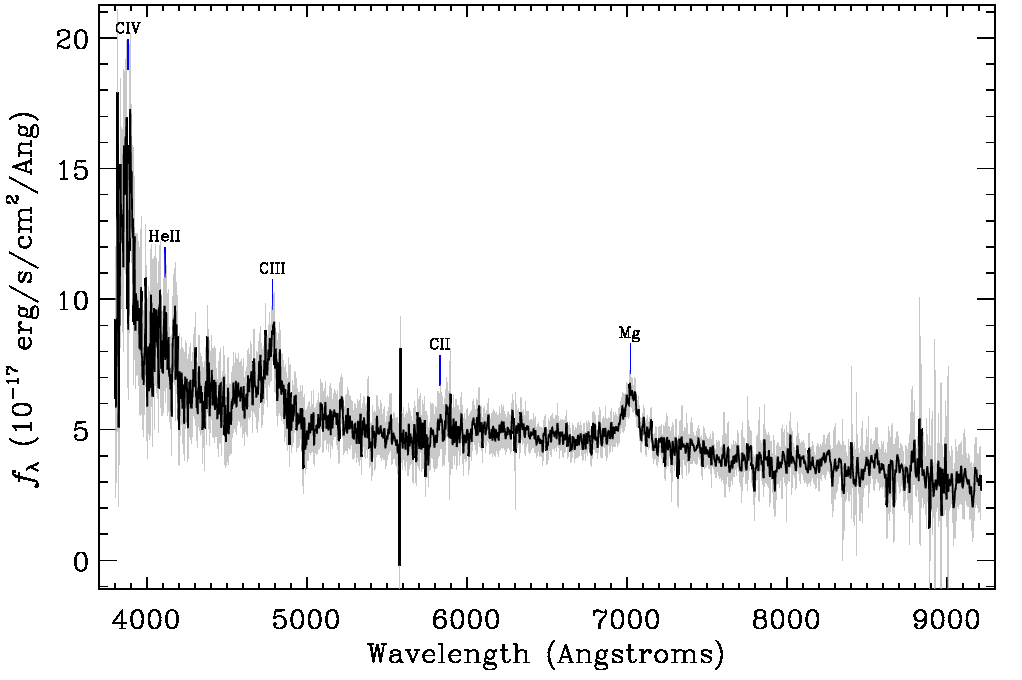
\includegraphics[scale=1]{spectra/j0843+2929_spectra_sdss.png}}
\caption{The spectrum of J0843+2929 taken by SDSS in 2003.}
\label{imbeded_fb}
\end{figure}



We find no evidence for the X-ray variability being associated with any particular physical characteristic. 
Therefore, we can link the variability to changes in the mass accretion rate. 
After it was observed with Einstein, its accretion rate decreased by a significant amount before its Chandra observation was taken in 2001.
Despite these dramatic changes, J0843+2929 is still a quasar and radiating at a high X-ray brightness.


\FloatBarrier




%%%%%%%%%%%%%%%%%%%%%%%%%%%%%%%%%%%
%%%%%%%%%%%%%%%%%%%%%%%%%%%%%%%%%%%%%
%%%%%%%%%%%%%%%%%%%%%%%%%%%%%%%%%%%%

\subsection{Source Luminosities}

As reported in Section 1.2, Seyfert galaxies have a typical luminosity value below 10$^{44}$ erg s$^{-1}$.
If an AGN has a luminosity higher than this, then it enters the range of luminosities typical to quasars.
Therefore, computing luminosity values for AGN can offer an additional diagnostic of their classification.
Thus, we report such values in table 4.1 for the 5 AGN presented above, where we calculate an X-ray luminosity using all available flux values for each source and distance measurements from NED.


%\begin{landscape}
    \begin{table}[h]
    \centering
    \scalebox{0.92}{
    \begin{tabular}{ccccc}
    \hline
    \hline
               source &        $z$  & L$_{\text{ETS}  }$ (erg s$^{-1}$)&  L$_{2\text{RXS}  }$ (erg s$^{-1}$)   &  L$_{\text{CSC}2.0  }$(erg s$^{-1}$) \\
               
    \hline
    
         J122934.1+134630 &     0.099 &  $1.1\times 10^{43}$ &  $1.3\times 10^{43}$ &  $1.6\times 10^{42}$ \\
        J111520.7+404326 &  0.079 &    $2.1\times 10^{43}$ &        $2.2\times 10^{42}$ &           $7.0\times 10^{42}$ \\
        J180117.9+662359 &  1.25 &     $3.8\times 10^{45}$ &         $1.2\times 10^{44}$ &           $1.6\times 10^{44}$ \\
        J082042.4+205715 &  0.11 &  $8.9\times 10^{42}$ &                  N/A & $8.4\times 10^{41}$ \\
        J084309.8+292919 &  1.51 & $3.9\times 10^{45}$  &                  N/A & $2.4\times 10^{44}$ \\
        \hline
        \hline
    \end{tabular}
    }
    \caption{Luminosity values of AGN with accretion-related variability.}
    \end{table}

%\end{landscape}




We see in Table 4.1 that no source crossed the 10$^{44}$ erg s$^{-1}$ luminosity boundary across its ETS, 2RXS, and CSC2.0 observation.
Thus, no source changed its Seyfert/quasar status.
We can use these luminosity values and the 10$^{44}$ erg s$^{-1}$ Seyfert/quasar boundary to classify J1229+1346, J1115+4043, and J0820+2057 as Seyferts.
This classification is consistent with their optical spectra, which also suggests they are Seyferts. 

We can make an additional additional diagnostic using the fact that narrow-line AGNs have a typical soft X-ray luminosity below $ 10^{43}$ erg s$^{-1}$ \citep{stocke1991}.
With this in mind, we see that J1229+1346 and J1115+4043 are potential CLAGN candidates since they cross this boundary.
Because we have a spectra of J1229+1346 during its $>10^{43}$ and $<10^{43}$ epochs, we can rule it out as a CLAGN candidate since its spectrum did not, in fact, change so much so that it is spectroscopically reclassified.
We would need a spectrum of J1115+4043 during its $>10^{43}$ epoch to truly determine it changed in its spectroscopic classification.

Finally, we see that J1801+6623 and J0843+2929 have luminosities greater than the $10^{44}$ Seyfert/quasar boundary.
This classifies them as quasars, which is consistent with their spectroscopic classification.





\FloatBarrier











%%%%%%%%%%%%%%%%%%%%%%%%%%%%%
%%%%%%%%%%%%%%%%%%%%%%%%%%%%%
%%%%%%%%%%%%%%%%%%%%%%%%%%%%%
%%%%%%%%%%%%%%%%%%%%%%%%%%%%%
%%%%%%%%%%%%%%%%%%%%%%%%%%%%%
%%%%%%%%%%%%%%%%%%%%%%%%%%%%%
%%%%%%%%%%%%%%%%%%%%%%%%%%%%%
%%%%%%%%%%%%%%%%%%%%%%%%%%%%%
%%%%%%%%%%%%%%%%%%%%%%%%%%%%%
%%%%%%%%%%%%%%%%%%%%%%%%%%%%%
%%%%%%%%%%%%%%%%%%%%%%%%%%%%%
%%%%%%%%%%%%%%%%%%%%%%%%%%%%%
%%%%%%%%%%%%%%%%%%%%%%%%%%%%%
%%%%%%%%%%%%%%%%%%%%%%%%%%%%%
%%%%%%%%%%%%%%%%%%%%%%%%%%%%%
%%%%%%%%%%%%%%%%%%%%%%%%%%%%%
%%%%%%%%%%%%%%%%%%%%%%%%%%%%%
%%%%%%%%%%%%%%%%%%%%%%%%%%%%%
%%%%%%%%%%%%%%%%%%%%%%%%%%%%%
%%%%%%%%%%%%%%%%%%%%%%%%%%%%%
%%%%%%%%%%%%%%%%%%%%%%%%%%%%%





\section{Non-Accretion Related X-ray Variability}

In the above section, we presented sources which had an X-ray variability likely related to accretion.
We also find sources in which the variability is not accretion related. 
In AGN, there can be a couple of different reasons for X-ray variability if not accretion related. 
The most common of reasons is due to radio-loud AGN, which characteristically display rapid, large amplitude variability due to relativistic beaming effects.
Types of radio-loud AGN that are subject to these effects are BL Lacertae objects and blazars.
Similarly, narrow-line Seyfert 1s also have a characteristic rapid variability in the X-ray that is not related to accretion.
The variability for these types of sources is a result of Compton scattering in the accretion disk \citep{mallick2018}.
A final way in which AGN can vary is due to variations in the absorption column densities associated with dust lanes or a dense dust torus, which can diminist the soft X-ray radiation coming from the nucleus along the line of sight.

Instrumentation differences can also create spurious X-ray variability in sources which might not have experienced any actual variability.
The most common scenario of this type is when observing galaxy clusters or groups.
The modest resolution afforded by the optics of Einstein and ROSAT did not allow them to resolve the discrete point sources within the cluster and in many cases, the extended emission associated with the cluster in nearly point-like.
Therefore, Einstein and ROSAT observed the cumulative and diffuse emission of the galaxy cluster.
Contrary to this, Chandra's fine resolution allows it to make out the discrete point sources within the galaxy cluster, and the point-source search algorithm employed in the construction of the CSC2.0 overlooks the extended emission.
Therefore, any variability associated with these types of observations is likely due to the different resolving power of the instruments and is likely not real.

Below, we present cases where we found highly variable X-ray emission, but after optically investigating the source, we find galaxies, AGN or other celestial objects that have X-ray variability that is not related to accretion.



\subsection{ J141314.8-031227}


J1413-0312, z = 0.0058, is a well known AGN by the name of NGC5506.
The ETS has a 0.5-2.0 keV flux of 5.55$\times 10^{-12}$ \fluxunits, the 2RXS observes a flux of 7.70$\times 10^{-13}$ \fluxunits, and the CSC2.0 reported a flux of 3.49$\times 10^{-14}$ \fluxunits.
This gives NGC5506 an ETS/2RXS flux ratio of 7.2, a 2RXS/CSC2.0 flux ratio of 22.05, and an ETS/CSC2.0 flux ratio of 158.9.
From all flux ratios, NGC5506 is considered a highly variable source.
It is also clear from the SDSS image and spectrum (show in figure 4.6ab that NGC5506 is a galaxy.
Specifically, it is classified as a Narrow Line Seyfert 1 (NLSy1) by \cite{nagar2002} because of the detection of the permitted OI$\lambda$1.1287$\mu$m line in its spectra (shown in fig 4.6a). 
This line is commonly produced in Seyfert 1s and never in Seyfert 2s.
Additionally, the detection of FeII lines at $\lambda$0.9997$\mu$m, $\lambda$1.0501$\mu$m, $\lambda$1.0863$\mu$m, and $\lambda$1.1126$\mu$m are argued to be produced from BLR clouds and are lines that have only been detected in six other extragalactic objects.
These six objects are also classified as NLSy1s.
NGC5506 also displays another important characteristic which is found in NLSy1s: X-ray variability.
This variability is likely due to the dust lanes found along the galactic disk \citep{nagar2002}.


\begin{figure}[h]
    \centering
    \subfloat[]{{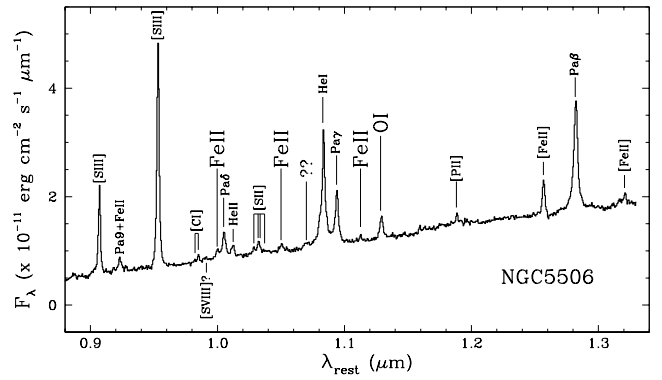
\includegraphics[width=10cm,height=6cm]{spectra/ngc5506_spectra_nagar_paper.png} }}%
    \qquad
    \subfloat[]{{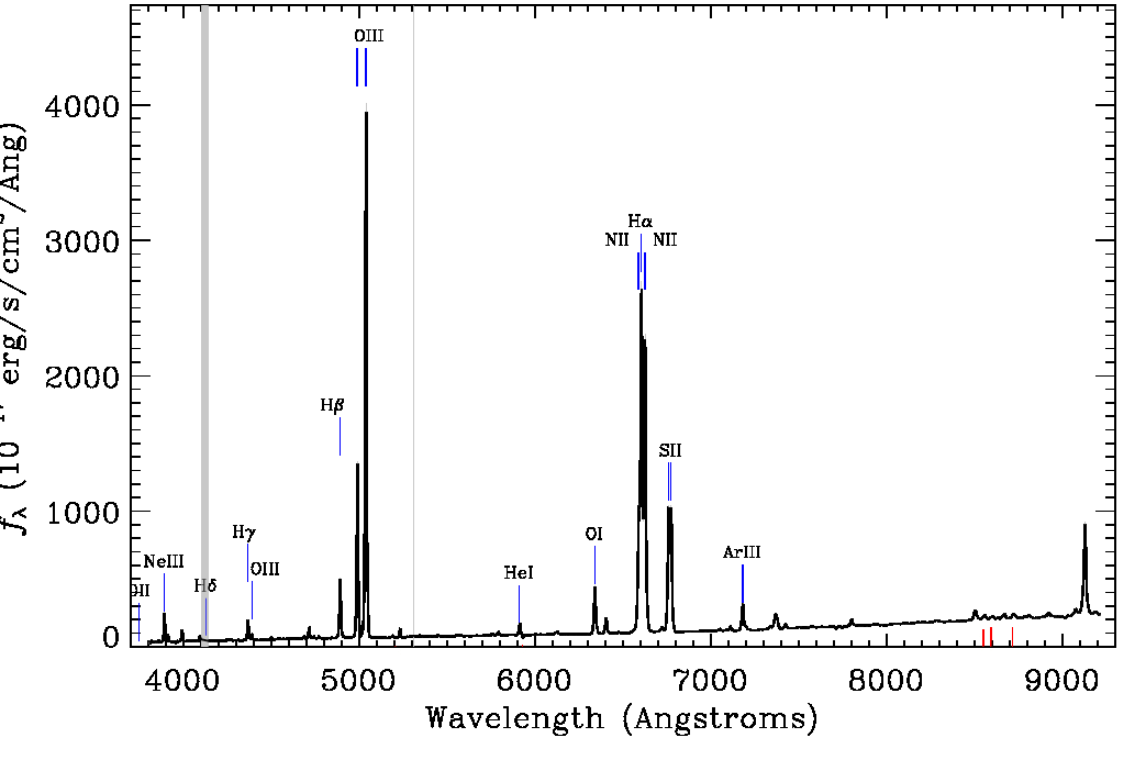
\includegraphics[width=10cm,height=6cm]{spectra/j1413-0312_spectra_sdss.png} }}%
    \caption{The spectrum of NGC5506 taken by \cite{nagar2002} in 2001 (a) and SDSS in 2002. }%
    \label{fig:example}%
\end{figure}





%\begin{figure}[h]
%\centering
%\scalebox{0.55}{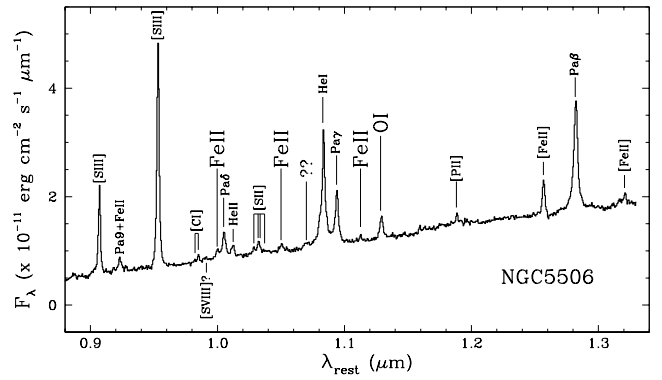
\includegraphics[scale=1]{spectra/ngc5506_spectra_nagar_paper.png}}
%\caption{The spectrum of NGC5506 taken by \cite{nagar2002} in 2001. }
%\label{imbeded_fb}
%\end{figure}

Because NGC5506 has an inclination of 70$^{\circ}$ and is close to being on edge, the dust in the galactic disk causes obscuration of the center, which complicates spectroscopic classifications. 
This has caused NGC5506 to be commonly classified as a type 1.9 or type 2 in the literature. 
This is the case in \cite{garcia2019} where it is classified as a type 1.9 Seyfert. 
In \cite{garcia2019}, NGC5506 is included in their sample of sources used to argue in favor of the AGN unification model. 
In this sample, which includes a total of 24 Seyferts, a torus for each object is modeled based on infrared photometry and spectroscopic measurements. 
Using the National Optical Astronomy Observatory’s (NOAO) CLUMPY, a program that models an AGN’s dust torus and its emission, \cite{garcia2019} derived torus properties for each object in its sample.
For NGC5506,  CLUMPY models the torus to have a bolometric luminosity of $\log(\text{L}_{\text{bol}}) = 43.86$,  a gas mass of 7.6 $\pm_{1.3}^{2.6}$ M$_{\odot}$, an outer radius of 3.8 $\pm_{0.3}^{0.6}$ pc and a torus covering factor of 0.91 $\pm_{0.02}^{0.01}$ \citep{garcia2019}. 
The torus’s bolometric luminosity and its covering factor are evidence for the X-ray variability being due to the dust absorption, as argued by \cite{nagar2002}.
Thus, the X-ray variability can not be directly credited to changes in NGC5506’s mass accretion rate changing.




%%%%%%%%%%%%%%%%%%%%%%%%%%%%%
%%%%%%%%%%%%%%%%%%%%%%%%%%%%%
%%%%%%%%%%%%%%%%%%%%%%%%%%%%%

\subsection{J140621.8+222346}


J1404+2223, z = 0.098, has an ETS 0.5-2.0 keV flux of 1.84$\times 10^{-13}$ \fluxunits, a 2RXS flux of 2.51$\times 10^{-12}$ \fluxunits, and a CSC2.0 flux of 9.17$\times 10^{-13}$ \fluxunits. 
This produces an ETS/2RXS flux ratio of 0.0733, a 2RXS/CSC2.0 ratio of 2.73, and an ETS/CSC2.0 ratio of 0.2. 
It is considered a highly variable X-ray source due to its ETS/2RXS flux ratio. 
J1404+2223 is a well studied source more commonly known as PG1404+226. 
From its SDSS spectra (shown in fig 4.7) and in the literature, PG1404+226 is classified as a NLSy1 \citep{mallick2018}. 
This is due to PG1404+226’s spectrum containing the common properties that define NLSy1s, whose spectra were measured and characterized by \cite{osterbrock1985}. 
The spectrum of PG1401+226 has strong permitted FeII emission lines and has a full width half maximum (FWHM) for H$\beta$ of less than 2,000 km s$^{-1}$. 
The FWHM of H$\beta$ for PG1404+226 is 787 km s${^-1}$ \citep{shangguan2018}.

\begin{figure}[h]
\centering
\scalebox{0.45}{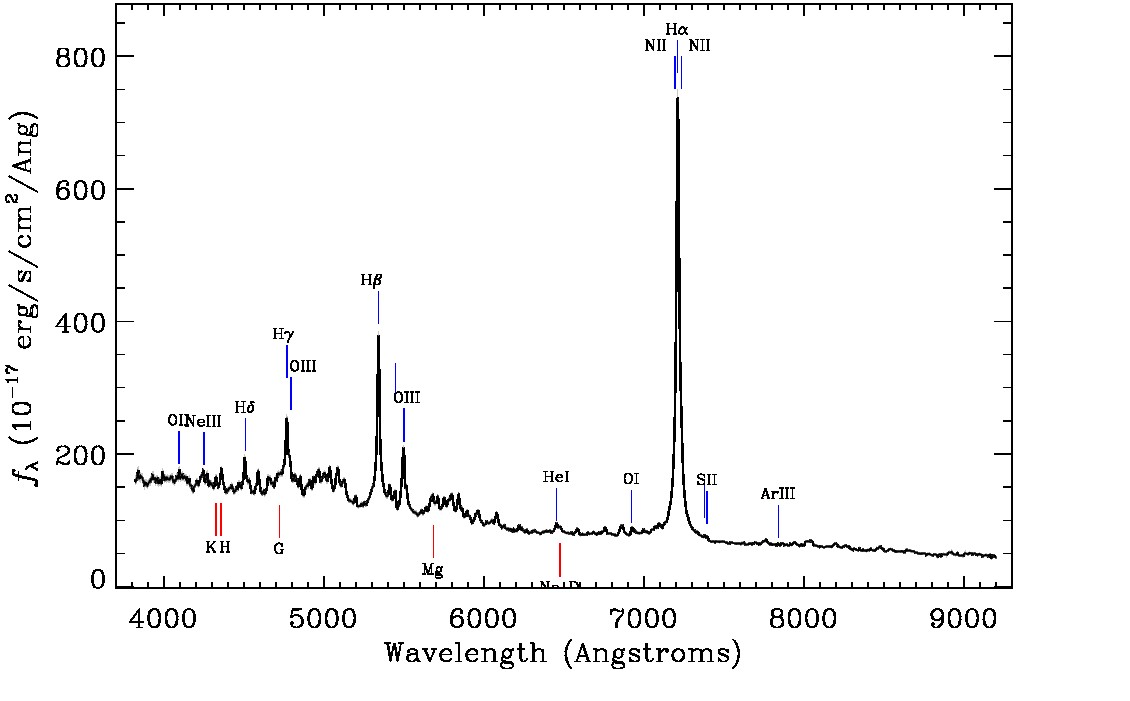
\includegraphics[scale=1]{spectra/j1406+2223_spectra_sdss.jpg}}
\caption{The spectrum of J1406+2223 from SDSS taken in 2008. }
\label{imbeded_fb}
\end{figure}

In \cite{shangguan2018}, the gas content of a sample of quasars are investigated; this sample includes PG1404+226.
Using data from the 2MASS, WISE, and Spitzer telescopes, they construct infrared spectral energy distributions (SEDS) for their sample.
From this, the emission of many physical components of the quasars (stellar, dust torus, dust from the ISM, and of jets for radio-loud quasars) are calculated. 
These properties are used as inputs in the CLUMPY program, which results in best-fit physical measurements.
For PG1404+226, CLUMPY estimates a mass of the dust of $\log(\text{M}_{ \text{d}  }  )$ = 7.89$\pm$ 0.03 M$_{\odot}$ and a mass of gas of $\log(\text{M}_{\text{g}}   )$ 9.99$\pm$0.20 M$_{\odot}$ \citep{shangguan2018}.

As is common in NLSy1s, PG1404+226 experiences large amplitude X-ray variability. 
In \cite{mallick2018}, PG1404+226 is observed to vary in its X-ray flux by a factor of 7 in only 10 ks. 
They hypothesize that this variability is due to variable opacity from the componization of the accretion disk and/or the relativistic reflection of the ionized accretion disk \citep{mallick2018}. 
Thus, the X-ray variability can not be directly credited to changes in PG1404+226’s mass accretion rate changing.

\FloatBarrier

%%%%%%%%%%%%%%%%%%%%%%%%%%%%%
%%%%%%%%%%%%%%%%%%%%%%%%%%%%%
%%%%%%%%%%%%%%%%%%%%%%%%%%%%%

\subsection{J135950.5+623105}

J1359+6231, z = 0.327, has an ETS 0.5-2.0 X-ray flux of 9.52$\times 10^{-13}$  \fluxunits, a 2RXS flux of 6.21$\times 10^{-13}$ \fluxunits and a CSC2.0 flux of 3.4$\times 10^{-14}$ \fluxunits. 
Therefore, it has an ETS/2RXS flux ratio of 1.53, a 2RXS/CSC2.0 flux ratio of 18.26, and an ETS/CSC2.0 flux ratio of 28. 
From its 2RXS/CSC2.0 and ETS/CSC2.0 flux ratios, J1359+6231 is considered a highly variable X-ray source.
Looking at the optical image (shown in fig 4.8) from SDSS makes it clear that this source is, in fact, a galaxy cluster. 

\begin{figure}[h]
\centering
\scalebox{0.60}{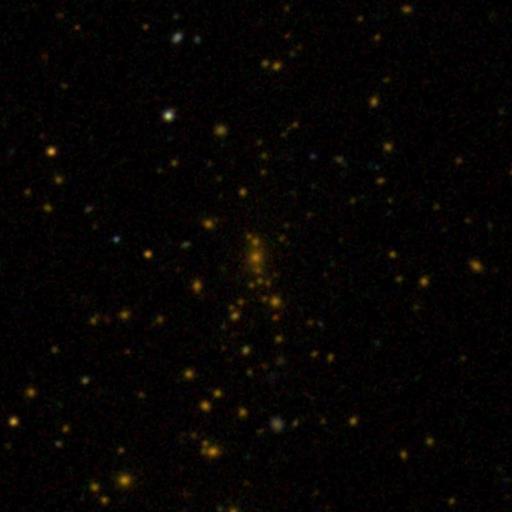
\includegraphics[scale=1]{images/j1359+6231_optical_img_sdss.jpg}}
\caption{The dense optical field around J1359+6231. }
\label{imbeded_fb}
\end{figure}


However, the broad H$\alpha$ line in the spectrum of one of its galaxies  (shown in fig 4.9) suggests that there is a possible AGN within the galaxy cluster. 
For this reason, J1359+6231 has frequently been included in studies which try to distinguish X-ray point sources and/or luminous X-ray galaxies within galaxy clusters. 
\cite{martini2009}, where J1359+6231 is referenced as ZwCl 1358.1+6245, looks for AGN in galaxy clusters to track the evolution of AGN as a function of redshift.
From observations at MDM, \cite{martini2009} find zero AGN with an X-ray luminosity greater than 10$^{43}$ erg s$^{-1}$ within J1359+6231. 
\cite{hart2009} additionally found 67 galaxies in the red sequence and only 1 radio-loud galaxy.

\begin{figure}[h]
\centering
\scalebox{0.60}{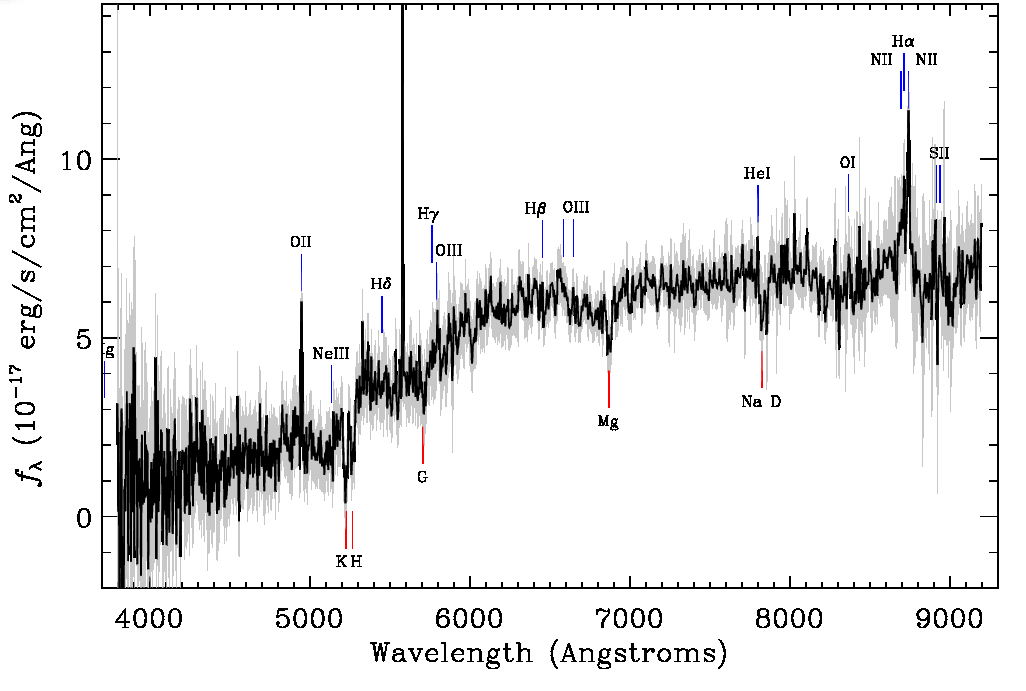
\includegraphics[scale=1]{spectra/j1359+6231_spectra_sdss.png}}
\caption{The spectrum of J1359+6231 taken by SDSS in 2002. }
\label{imbeded_fb}
\end{figure}

There is no evidence for a physical feature being responsible for the variability in the X-ray flux and that is likely because it is not due to a physical feature.
Instead, it is likely that Einstein and ROSAT observed the diffusive emission of the galaxy cluster which must be much greater than the luminosity of the AGN in it while Chandra was able to observe just one of the galaxies from the cluster.
Therefore, the variability can not be attributed to a change in mass accretion rate of a particular AGN.


\FloatBarrier

%%%%%%%%%%%%%%%%%%%%%%%%%%%%%
%%%%%%%%%%%%%%%%%%%%%%%%%%%%%
%%%%%%%%%%%%%%%%%%%%%%%%%%%%%



\subsection{J090720.5+163906}

J0907+1639, z = 0.072,  has an ETS 0.5-2.0 X-ray flux of 5.65$\times 10^{-13}$ \fluxunits, a 2RXS flux of 8.28$\times 10^{-13}$ \fluxunits and a CSC2.0 flux of 2.10$\times 10^{-14}$ \fluxunits. 
This produces an ETS/2RXS flux ratio of 0.682, a 2RXS/CSC2.0 flux ratio of 39.44, and an ETS/CSC2.0 flux ratio of 26.92. 
From its 2RXS/CSC2.0 flux ratio and ETS/CSC2.0 flux ratio, J0907+1639 is considered a highly variable X-ray source. 
The SDSS image and spectrum (shown below in fig 4.10) suggests the source is a regular, elliptical galaxy.
However, upon closer examination, this source is, in fact, a galaxy cluster. 
More specifically, J0907+1639 is classified as a fossil cluster --- a galaxy cluster or group that is dominated by a giant elliptical galaxy at its center \citep{veovodkin2010}. 
Using data from the SDSS-DR13, \cite{omill2019} finds spectroscopic and photometric data for any member of the cluster and determines that J0907+1639 is a low X-ray luminosity galaxy cluster. 
With spectra  collected for 19 members and photometric measurements are found for 32 members, an X-ray luminosity of 0.34$\pm 0.03 \times 10^{44}$ erg s$^{-1}$ is calculated \citep{omill2019}.


\begin{figure}[h]
    \centering
    \subfloat[]{{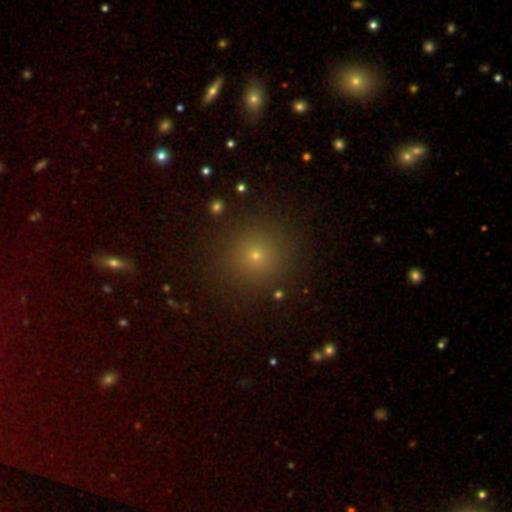
\includegraphics[scale=0.4]{images/j0907+1639_optical_img.jpg} }}%
    \qquad
    \subfloat[]{{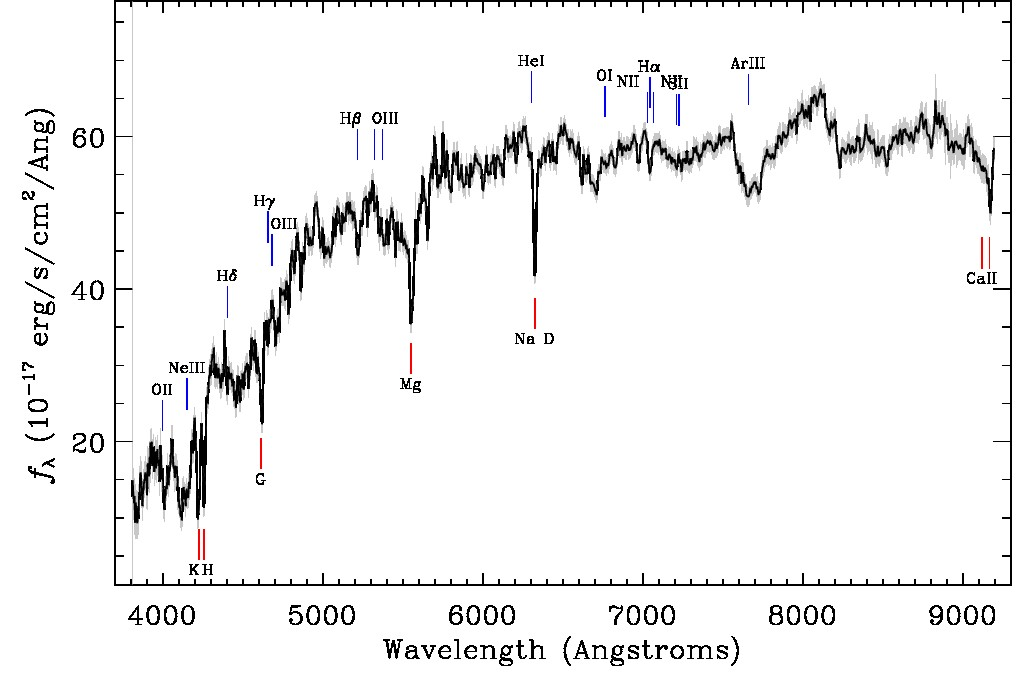
\includegraphics[scale=0.4]{spectra/j0907+1639_spectra_sdss.jpg} }}%
    \caption{The optical field around J0907+1639 showing a dense field of galaxies (a) and J0907+1639's SDSS spectrum (b) taken in 2006 and exhibits no emission-line activity. }%
    \label{fig:example}%
\end{figure}


%\begin{figure}[h]
%\centering
%\scalebox{0.47}{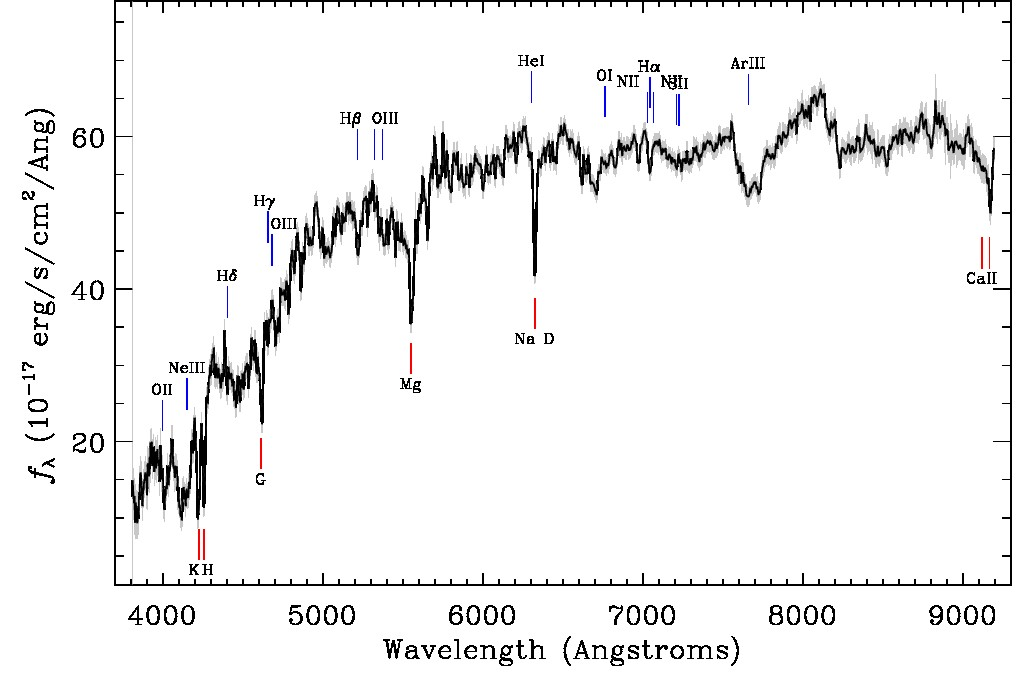
\includegraphics[scale=1]{spectra/j0907+1639_spectra_sdss.jpg%}}
%\caption{The spectrum of J0907+1639 from SDSS. }
%\label{imbeded_fb}
%\end{figure}

No evidence for any physical feature being responsible for the variability in the X-ray flux is found. 
We conclude that the variability is must be spurious. 
Instead, the variability is likely due to the differing optics in the telescopes used. 
That is, Einstein and ROSAT likely observed the diffuse emission of the entire galaxy cluster while Chandra observed only the elliptical at the center. 

\FloatBarrier

%%%%%%%%%%%%%%%%%%%%%%%%%%%%%
%%%%%%%%%%%%%%%%%%%%%%%%%%%%%
%%%%%%%%%%%%%%%%%%%%%%%%%%%%%


\subsection{ J011853.6-010007}



J0118-0100, z = 0.045, is more commonly known as UGC00842. 
It has a 0.5-2.0 X-ray fluxes of 3.92$\times 10^{-13}$ \fluxunits, 2.58$\times 10^{-13}$ \fluxunits, and 1.86$\times 10^{-14}$ \fluxunits calculated from the ETS, 2RXS, and CSC2.0, respectively. 
These values give an ETS/2RXS flux ratio of 1.52, a 2RXS/CSC2.0 flux ratio of 13.88, and an ETS/CSC2.0 flux ratio of 21.09. 
UGC00842 is classified as a highly variable X-ray source due to its 2RXS/CSC2.0 flux ratio and ETS/CSC2.0 flux ratio. 
The SDSS spectrum (shown in fig 4.11) of UGC00842 presents weak emission lines and stellar absorption lines from the stars within the galaxy.
The rather featureless spectrum does not initially suggest the presence of any nuclear activity. 
Radio emission, however, has been detected in UGC00842, which has made it an interesting source to conduct follow up studies on. 
In \cite{brinkmann2000}, which set out to find bright radio and X-ray galaxies by cross correlating the ROSAT All-Sky Survey with the VLA 20cm FIRST Catalog, UGC00842 is found in the cross-correlation and is confirmed to be a BL Lacertae (BL Lac). 
BL Lac are radio-loud AGN characterized by their featureless spectrum with weak emission lines and stellar absorption features, much like spectrum of UGC00842 \citep{falomo2014}.


\begin{figure}[h]
\centering
\scalebox{0.60}{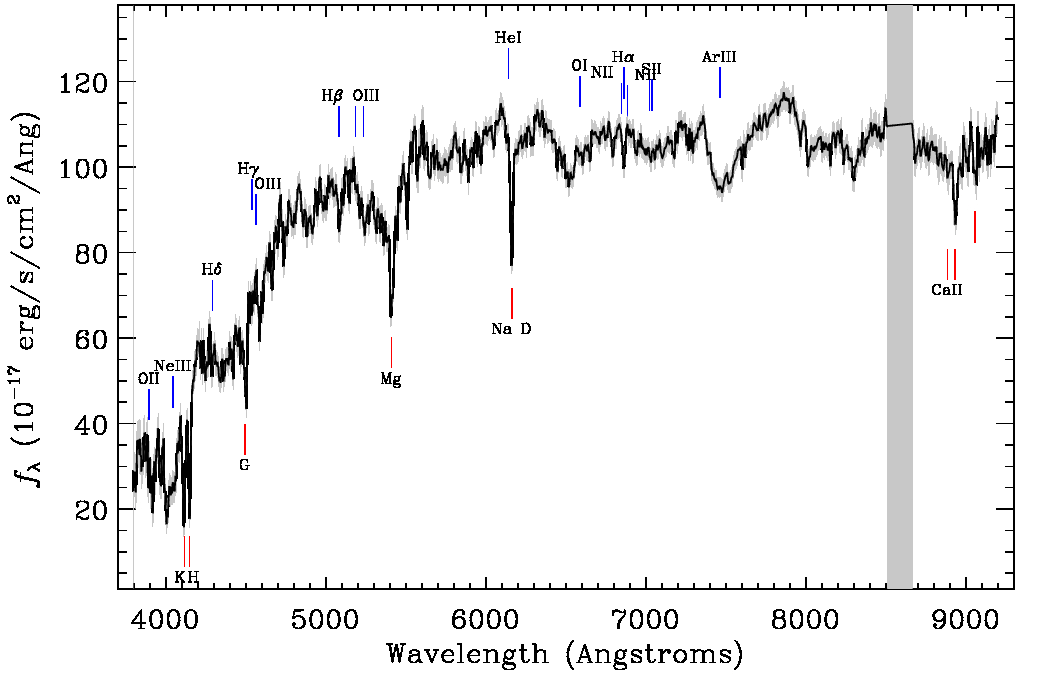
\includegraphics[scale=1]{spectra/j0118-0100_spectra_sdss.png}}
\caption{The spectrum of J0118-0100 taken by SDSS in 2000.}
\label{imbeded_fb}
\end{figure}

Another important characteristic found in BL Lac objects is the large amplitude flux variability present over much of the electromagnetic spectrum. 
In other AGN, X-ray variability can be linked to the accretion rate. 
In BL Lac objects, however, this association can not be made since flux variability is known to be caused by the relativistic beaming of jets stemming from the nucleus.
Therefore, we do not find a change in the accretion rate of UGC00842’s accretion disk.


\FloatBarrier
%%%%%%%%%%%%%%%%%%%%%%%%%%%%%
%%%%%%%%%%%%%%%%%%%%%%%%%%%%%
%%%%%%%%%%%%%%%%%%%%%%%%%%%%%




\subsection{J011515.7+001248}

J0115+0012, z = 0.045, has an ETS 0.5-2.0 X-ray flux of $3.8\times 10^{-13}$ \fluxunits and a CSC2.0 flux of 2.99$\times 10^{-14}$ \fluxunits. 
This produces an ETS/CSC2.0 flux ratio of 12.7, which classifies it as a variable X-ray source. 
The SDSS spectrum for J0115+0012 (shown in fig 4.12 alongside its optical field) suggests it is an AGN due to the broad H$\alpha$ emission line and strong [NII] lines.
The spectrum also displays stellar absorption features. 
While J0115+0012’s spectrum doesn’t hint at any other interesting optical characteristics, J0115+0012 turns out to be a fairly well-studied source, more commonly known as GIN 061. 
GIN 061 was first observed to be the brightest source within galaxy cluster ABELL 0168 \citep{faber1977}. 
Follow up studies on GIN 061 found that it is also a radio-loud galaxy after conducting observations with the JVLA \citep{baldi2015}. 




\begin{figure}[h]
    \centering
    \subfloat[]{{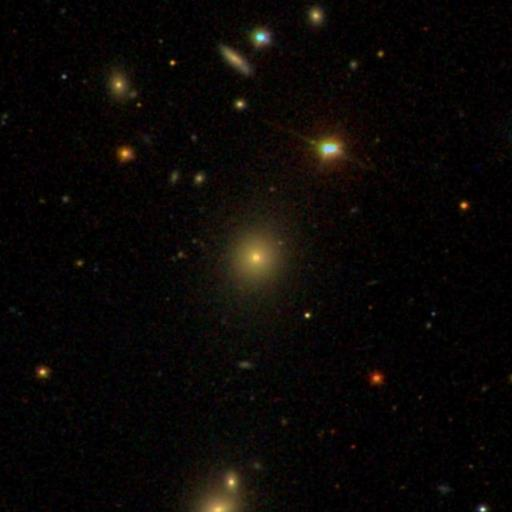
\includegraphics[scale=0.43]{images/j0115+0012_optical_img.jpg} }}%
    \qquad
    \subfloat[]{{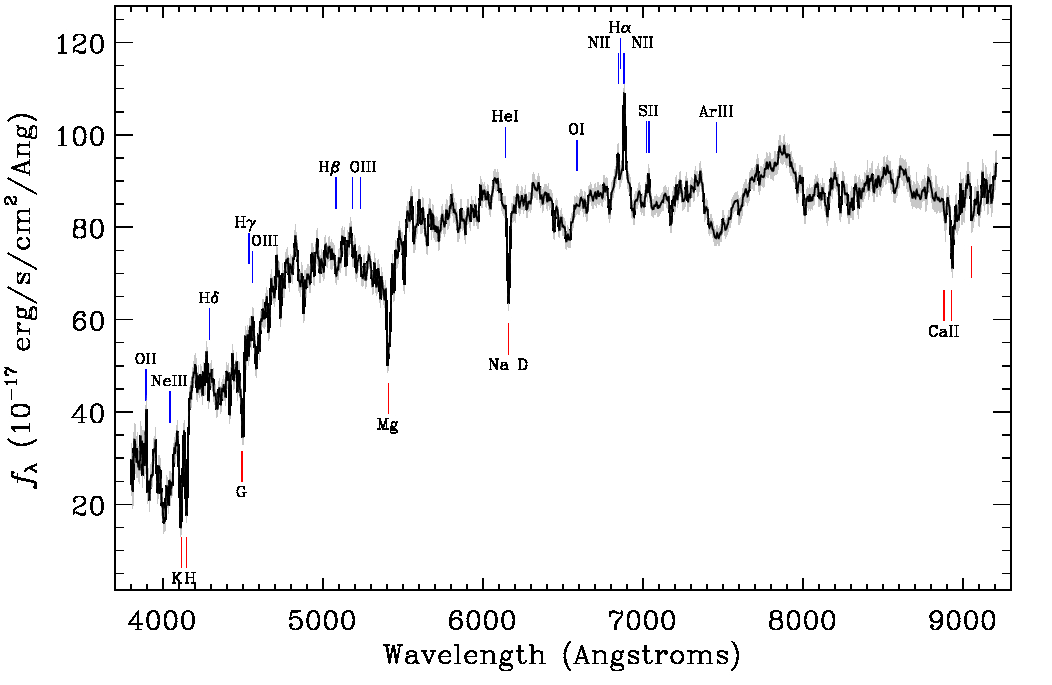
\includegraphics[scale=0.43]{spectra/j0115+0012_spectra_sdss.png} }}%
    \caption{The optical field around J0115+0013 ABELL 0168 (a) and J0907+1639's spectrum taken by SDSS in 2000 (b). }%
    \label{fig:example}%
\end{figure}



%\begin{figure}[h]
%\centering
%\scalebox{0.55}{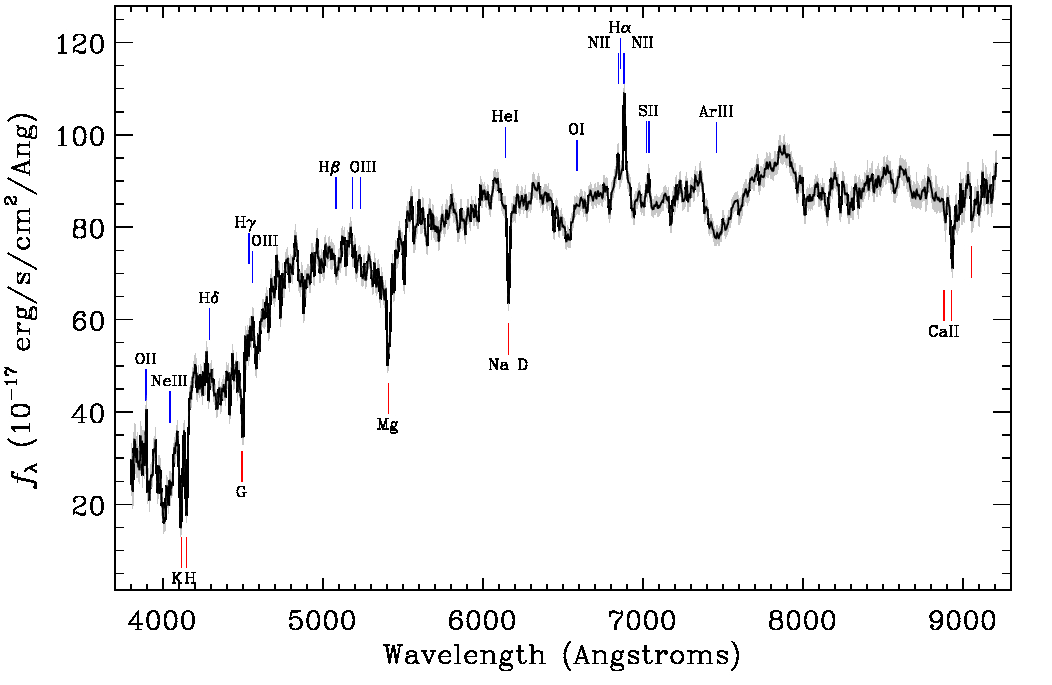
\includegraphics[scale=1]{spectra/j0115+0012_spectra_sdss.png}}
%\caption{The spectrum of J0115+0012 from SDSS.}
%\label{imbeded_fb}
%\end{figure}



\cite{baldi2015} conducted an X-ray study on their 2015 sample of radio galaxies, where GIN 061 and its host cluster were included.
They found that the cluster itself had many sources that are bright in the X-ray in addition to being radio-loud. 
This suggests that the X-ray variability observed is likely an artifact of the telescope optics. 
That is, the Einstein telescope likely observed the diffuse emission of the galaxy cluster as well as the sum of the many X-ray sources confirmed in \cite{baldi2015}.
On the other hand, Chandra’s fine angular resolution allowed it to observe the X-ray emission radiating only from GIN 061. 
For this reason, the variability observed is not due to a change in the mass accretion rate of the source.


\FloatBarrier


%%%%%%%%%%%%%%%%%%%%%%%%%%%%%
%%%%%%%%%%%%%%%%%%%%%%%%%%%%%
%%%%%%%%%%%%%%%%%%%%%%%%%%%%%


\subsection{J132117.8+423515}

J1231+4235, z = 0.79, has an ETS flux of 7.23$\times 10^{-14}$  \fluxunits and CSC2.0 flux of 1.70$\times 10^{-15}$ \fluxunits in the 0.5-2.0 keV band. 
This gives rise to an ETS/CSC2.0 flux ratio of 42.6. 
The SDSS spectrum (fig 4.13) has narrow H$\alpha$ and H$\beta$ emission lines and a strong OIII line. 
Some stellar absorption features are apparent, as well.
With an OIII line much stronger than the H$\beta$ line, J1321+4235 can be classified as an AGN.
J1321+4235 is a well-studied source more commonly known as 3C 285 and long-confirmed as a narrow line AGN \citep{fabiano1984}. 
3C285, however, is also a low excitation radio galaxy (LERG), with a straight jet length of 72 kpc \citep{krause2019}.

\begin{figure}[h]
\centering
\scalebox{0.55}{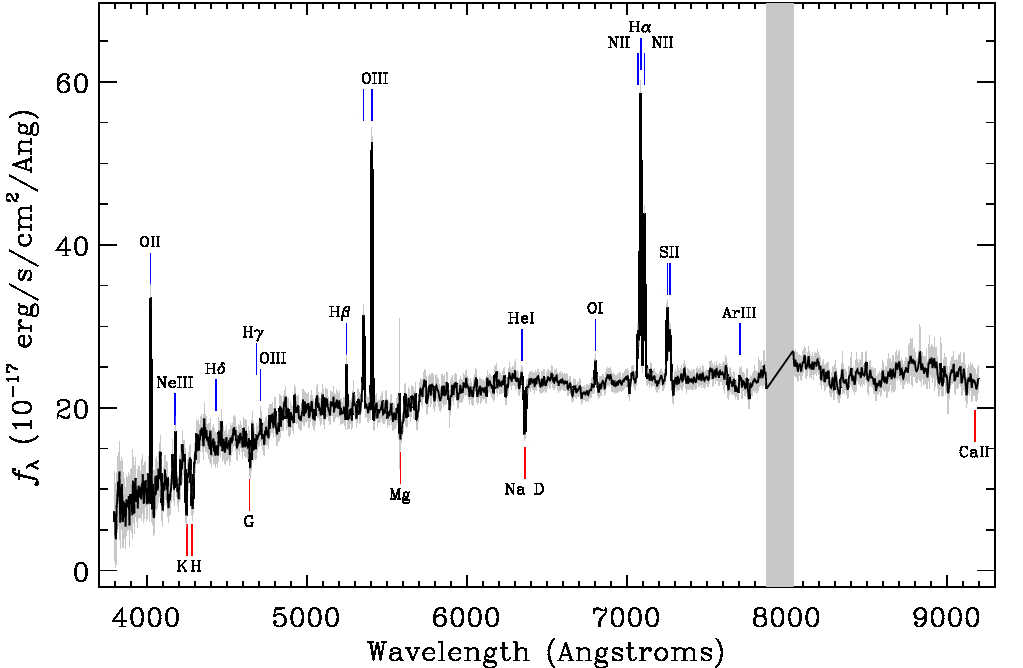
\includegraphics[scale=1]{spectra/j1321+4235_spectra_sdss.png}}
\caption{The spectrum of J1321+4235 from SDSS takn in 2004.}
\label{imbeded_fb}
\end{figure}


A distinctive feature in LERGS is that they have a different kind of accretion mode. 
In standard AGN, cold matter from a disk is accreted onto the SMBH in an efficient fashion.
This mode radiates energy across the electromagnetic spectrum. In LERGS however, accretion is believed to happen in a “hot mode”.
That is, rather than cold matter accreting onto the SMBH, hot gas is being accreted. 
This process is radiatively inefficient and results in little radiated energy, but can produce radio jets, as is the case for 3C285 \citep{best2012}. 
Because of the “hot mode” accretion, no X-ray or IR emission is produced from the accretion \citep{hardcastle2007}. 
Therefore, the X-ray variability in 3C285 is not due to a change in its accretion rate. Rather, because it is a radio source, the variability is likely caused by relativistic beaming effects.

\section{Untangled Multiple Matches}


Following the procedure laid out in Section 3.5.2, we can assess for variability of sources that matched to 2 CSC2.0 sources. Due to our assumptions and the complexity of the scenario, we can have some level or reliability in our findings but must be careful with the interpretation of the variability. Below, we present 1 source that demonstrates high X-ray variability and is found in the SDSS.

\subsection{J083052.2+241056}


J0830+2410, z = 0.938, was one of two CSC2.0 sources that matched a singular 2RXS source. Subtracting the flux of the other CSC2.0 source from the ETS and 2RXS source flux gives values of 3.9$\times 10^{-13}$ \fluxunits and 8.7$\times 10^{-13}$ \fluxunits, respectively. 
The CSC2.0 flux for J0830+2410 is 3.1$\times 10^{-14}$ \fluxunits. 
Therefore, the ETS/2RXS, ETS/CSC2.0, and 2RXS/CSC2.0 flux ratios are 0.44, 28.2, and 12.5, respectively. 
This classified J0830+2410 as a highly variable AGN. From its SDSS spectrum (shown in fig 4.14), it is clear that the source is a quasar. 
The spectrum has a steep power law continuum with broad Mg and H$\gamma$, all which are characteristic of a quasar.
J0830+2410 is in fact, a very well known and well studied source with multiple confirmations of it being a blazar \citep{arsioli2018}. 
These types of sources are known for being radio loud and having relativistic beaming along the line of sight. Blazars are characterized by their flat radio spectrum, which \cite{healey2007} observed J0830+2410 to have.


\begin{figure}[H]
\centering
\scalebox{0.52}{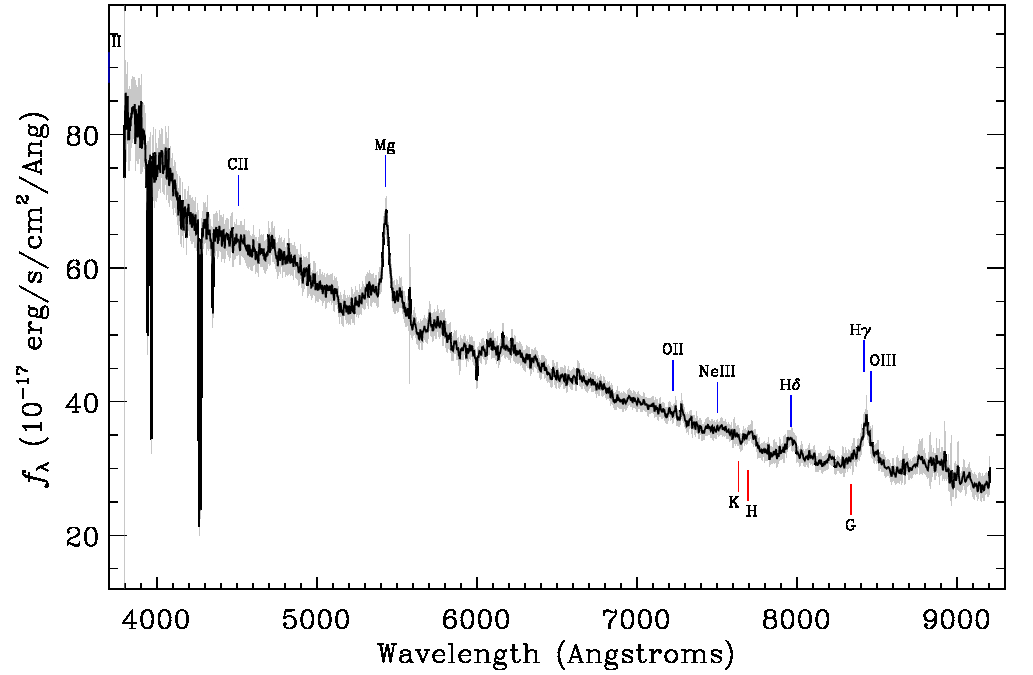
\includegraphics[scale=1]{spectra/j0830+2410_spectra_sdss.png}}
\caption{The spectrum of J0830+3410 taken by SDSS in 2004.}
\label{imbeded_fb}
\end{figure}

Radio sources, and particularly blazars, are known for their high variability, which drowns out much of the thermal radiation from the nucleus. 
Therefore, any X-ray variability that is observed is likely not related to accretion changes. 
Under the assumption that the variability is entirely due to this source and not the other CSC2.0 counterpart that matched to the 2RXS source, the X-ray change can be associated with relativistic beaming effects.


\FloatBarrier
\chapter{Discussion}
\label{chap5}

\section{Summary}
\label{sub5_1}

We have described the process for which we cross-correlated sources between the ETS, 2RXS, and CSC2.0, which allowed for a direct comparison of their 0.5-2.0 X-ray fluxes. 
Using a threshold of 7, we have constructed a sample of variable X-ray sources (Chapter 3). 
We optically investigated this sample through the SDSS and careful literature review.
From the 12 sources that were observed and had optical spectra in SDSS, we have determined that 5 AGN have experienced a dramatic change in their X-ray variability that is due to changes in their mass accretion rate. 
These 5 AGN all dimmed in brightness somewhere between Einstein and Chandra observations. 
On the other hand,  we concluded that the X-ray variability of the other t sources is not accretion related. 
The reasons for non-accretion related X-ray variability ranged from relativistic beaming of radio-loud galaxies to observed diffuse emission from galaxy clusters (Chapter 4).


\section{Big Picture}
\label{sub5_2}



Because changes in the accretion state of AGN are events that occur on cosmic timescales, they are rare events to observe given our limited baseline provided by the history of imaging X-ray Astronomy. 
The results presented here reinforce that since, in the end, we find only five AGN that potentially have had major changes in their accretion state. 
However, the limitation on our results is not solely due to the cosmic timescale of these events. 
The need to have multiple observations of the same source at different epochs is a major limiting factor on our results. 
We made use of observations from three X-ray telescopes: Einstein, ROSAT, and Chandra. 
Each has its own distinct footprint, which do not necessarily overlap extensively in some parts of the sky. 
The sources available for investigation for this project are those found in the intersection of their footprints. 
This limits extensively the amount of data that can be considered for this project. 
Another major cut is made to the data available for consideration when looking for optical follow-up data in the SDSS. 
Without corresponding optical data, there is not much that can be done to investigate the nature of the source producing the X-ray emission. 
All these factors play a significant role in limiting our search for changes in the accretion state of AGN.

Nonetheless, our results motivate the continuation of the search of these types of objects.
Finding more of them and creating a more extensive sample, we can begin to find patterns that potentially {\it explain\/} the changes in accretion states. 
Specifically, we can begin to compare the optical morphologies of the variable sources to those of non-variable AGNs using high-resolution imaging. 
Over a considerable amount of time, we can potentially find trends in how galaxy morphologies are related to the activity in the galactic center.  
We can also begin to explore the environments of the galaxies and the environments around the galaxy centers. 
This can help identify patterns that link changes in accretion state to some property related to its host galaxy. In doing this, we are inspecting the conditions which directly affect BH fueling.

\section{Future Work}


We want to continue to monitor the status of the five AGN observed to potentially have a change in their accretion rate. 
We see that the last Chandra observations for all five sources occured in the early to mid- 2000s, more than fifteen years ago now for most of these sources.
A Chandra follow up conducted now will reveal their current X-ray flux standing, and an optical follow up will offer a modern spectroscopic classification of these objects. 
We want to follow a similar procedure for the variable X-ray sources that did not have an SDSS observation. 
This can increase our sample if more AGN with accretion-related X-ray variability are found. 
Along with adding new data to our existing sample of X-ray variable AGN, we can also look back at X-ray data archives and conduct an extensive search for serendipitous observations that could fill in the gaps between the Einstein, ROSAT, and Chandra observations. 
A more complete light curve can restrict the era in which the change in accretion states occurred. 
It will similarly help solidify these events as long-term processes.



\subsection{New Era of Sky Surveys}

With the continuous advances in technology, new telescopes that possess increasing capabilities will emerge.
Two such telescopes that will surely benefit a project like this are the extended R\"{o}ntgen Survey with an Imaging Telescope Array (eROSITA) X-ray Observatory and the Vera C. Rubin Observatory (previously known as the Large Synoptic Survey Telescope).

The eROSITA, which launched on July 13, 2019, will conduct an All Sky Survey (called the eROSITA All-Sky Survey or eRASS) in the 0.2-10 keV energy band in similar fashion to the RASS.
That is, eRASS will also scan the sky with a rotation axis in the plane of the Earth' orbit, which will create great circles that overlap at the ecliptic poles. 
In this 4 year survey, the full sky will be observed every 6 months, leading to 8 total passes of the sky in 4 year survey. 
In the 0.5-2.0 keV soft X-ray band, the eRASS will be roughly 20 times more sensitive than the RASS. 
This will result in an expected detection of 10,000 galaxy clusters and 3 million AGN, greatly increasing the population of known X-ray sources \citep{merloni2012}.

Optically, the Vera C. Rubin Observatory will conduct the Legacy Survey of Space and Time (LSST) over 10 years, which will cover 18,000$^{\circ}$ of southern hemisphere sky.
This will complement the SDSS's northern hemisphere survey. 
While the LSST is primarily focused on observing objects within the Milky Way, it is still projected to observe 20 billion galaxies \citep{ivezi2019}.

Future iterations of this project will have a larger amount of X-ray data and greater potential of optically identifying the sources because of these surveys. 
The eRASS and the LSST will provide an enormous amount of new data that will aid in exposing the true nature of black hole fueling. 


%-----------------------------------------------------------------------------------------------------------------------------------------
%% APPENDIX

%tell LaTeX that you're now in the appendix section:

%\appendix

%I wanted my title formatting to be slightly different here, so that things are numbered "Appendix A" instead of "Chapter A" or "Chapter 6"

% \titleformat{\chapter}{\bf\huge}
% {Appendix \thechapter}{-5.35em}{\\}
% \titlespacing*{\chapter}{0pt}{-.5in}{*3}

% %These are the file names of my appendices:
% \include{Distance_Code}
% \include{Spectroscopy}
% \include{LINERs}

\doublespacing


%-----------------------------------------------------------------------------------------------------------------------------------------
%%BIBLIOGRAPHY:

\fancypagestyle{plain}{%
% clear all header and footer fields, we don't want these for the bibliography
\fancyhf{} 
% except we want the page number to show up in the center of the footer:
\fancyfoot[C]{\thepage} 

\renewcommand{\headrulewidth}{0pt}
\renewcommand{\footrulewidth}{0pt}}
\pagestyle{plain}

%change title spacing once again, for the bibliography:
\titlespacing*{\chapter}{0pt}{-.75in}{*3}

%Add the bibliography to the table of contents, it doesn't show up by default, you have to specify it:
\addcontentsline{toc}{chapter}{\textbf {Bibliography}}

%The default for BibTex (the bibliography builder in LaTeX) is to not include citations that are in your bibliography file, but that you don't cite anywhere in the paper.  This changes that setting, so that all papers show up in the bibliography, whether or not you referenced them:
\nocite{*}

%Insert the bibliography (in this case, my file name was also "bibliography" if not, your line would read: \bibliography{my_workscited_filename} or whatever:
\bibliographystyle{apj}
\bibliography{bibliography}

%the end!
\end{document} 